% ============================================================
%  Airbnb Paris — Optimal Pricing Prediction
%  Business Analytics — HEC Paris, May 2026
%  12-minute Beamer presentation
% ============================================================
\documentclass[aspectratio=169, 10pt]{beamer}

\usetheme{metropolis}
\usepackage{appendixnumberbeamer}
\usepackage{booktabs}
\usepackage{tikz}
\usetikzlibrary{positioning, arrows.meta}
\usepackage{xcolor}
\usepackage{fontawesome5}
\usepackage{colortbl}
\usepackage{array}
\usepackage{graphicx}
\usepackage{microtype}
\usepackage[utf8]{inputenc}
\usepackage[T1]{fontenc}

% ── Colours ──────────────────────────────────────────────────
\definecolor{airbnbCoral}{HTML}{FF5A5F}
\definecolor{airbnbDark}{HTML}{484848}
\definecolor{airbnbGrey}{HTML}{767676}
\definecolor{airbnbLight}{HTML}{F7F7F7}
\definecolor{airbnbTeal}{HTML}{00A699}
\definecolor{clusterRed}{HTML}{E74C3C}
\definecolor{clusterBlue}{HTML}{3498DB}
\definecolor{clusterGreen}{HTML}{2ECC71}
\definecolor{clusterOrange}{HTML}{F39C12}

\setbeamercolor{frametitle}{bg=airbnbCoral, fg=white}
\setbeamercolor{progress bar}{fg=airbnbCoral, bg=airbnbLight}
\setbeamercolor{title separator}{fg=airbnbCoral}
\setbeamercolor{alerted text}{fg=airbnbCoral}
\setbeamercolor{block title}{bg=airbnbCoral!15, fg=airbnbDark}
\setbeamercolor{block body}{bg=airbnbLight, fg=airbnbDark}
\setbeamercolor{normal text}{fg=airbnbDark}

\metroset{block=fill, progressbar=frametitle, sectionpage=progressbar,
          numbering=fraction}

% Fix overfull vbox on auto-generated section pages (pages 3, 9, …):
% replace fixed minipage with flexible vfill so the content never exceeds frame height.
\setbeamertemplate{section page}{%
  \vspace*{0pt plus 1fill}%
  \centering
  \begin{minipage}{22em}
    \raggedright
    \usebeamercolor[fg]{section title}%
    \usebeamerfont{section title}%
    \insertsection\par
    \usebeamertemplate*{progress bar in section page}%
  \end{minipage}%
  \par
  \vspace*{0pt plus 1fill}%
}

\newcommand{\hl}[1]{\textcolor{airbnbCoral}{\textbf{#1}}}
\newcommand{\tl}[1]{\textcolor{airbnbTeal}{\textbf{#1}}}

\graphicspath{{./plots/}{./}}

\title{Optimal Pricing Prediction\\for Airbnb Listings in Paris}
\subtitle{Business Analytics Using Python --- HEC Paris}
\author{Group Project}
\date{May 2026}

% ============================================================
\begin{document}
% ============================================================

% ── 1. Title ─────────────────────────────────────────────────
{
\setbeamercolor{background canvas}{bg=airbnbDark}
\begin{frame}[plain]
  \vspace{0.7cm}
  {\color{airbnbCoral}\rule{\textwidth}{2pt}}\\[0.3cm]
  {\color{white}\LARGE\textbf{Optimal Pricing Prediction}}\\[0.15cm]
  {\color{white}\Large for Airbnb Listings in Paris}\\[0.5cm]
  {\color{airbnbLight}\small Business Analytics Using Python
    $\cdot$ HEC Paris $\cdot$ May 2026}
  \vfill
  \begin{columns}[T]
    \column{0.24\textwidth}\begin{block}{}\centering
      {\color{airbnbCoral}\Large\textbf{64\,690}}\\[-2pt]\small Paris listings\end{block}
    \column{0.24\textwidth}\begin{block}{}\centering
      {\color{airbnbCoral}\Large\textbf{8}}\\[-2pt]\small models trained\end{block}
    \column{0.24\textwidth}\begin{block}{}\centering
      {\color{airbnbCoral}\Large\textbf{R\textsuperscript{2}=0.66}}\\[-2pt]\small best model\end{block}
    \column{0.24\textwidth}\begin{block}{}\centering
      {\color{airbnbCoral}\Large\textbf{4}}\\[-2pt]\small listing segments\end{block}
  \end{columns}
  \vspace{0.4cm}
  {\color{airbnbCoral}\rule{\textwidth}{2pt}}
\end{frame}
}

% ── 2. Roadmap ───────────────────────────────────────────────
\begin{frame}{Roadmap \& Core Question}
  \begin{columns}[T]
    \column{0.52\textwidth}
    \begin{enumerate}
      \setlength{\itemsep}{0.4em}
      \item[\hl{1.}] Business problem \& dataset
      \item[\hl{2.}] Exploratory data analysis
      \item[\hl{3.}] Feature engineering \& selection
      \item[\hl{4.}] Supervised models --- all 8 compared
      \item[\hl{5.}] Classification into price tiers
      \item[\hl{6.}] Amenity analysis \& decision tree
      \item[\hl{7.}] Unsupervised segmentation (K-Means)
      \item[\hl{8.}] Business recommendations
    \end{enumerate}
    \column{0.46\textwidth}
    \begin{block}{Core question}
      \small What are the \textbf{key drivers} of Airbnb listing prices
      in Paris, and can we build a \textbf{reliable predictive model}
      to help hosts set an optimal price?
    \end{block}
    \vspace{0.25cm}
    \begin{block}{Data}
      \small Inside Airbnb --- 10-city snapshot\\
      \textbf{64\,690 Paris listings}, 5.4M reviews\\
      20 neighbourhoods $\cdot$ License: CC0
    \end{block}
  \end{columns}
\end{frame}

% ============================================================
\section{Business Problem \& Dataset}
% ============================================================

\begin{frame}[shrink=3]{Business Problem \& Dataset at a Glance}
  \begin{columns}[T]
    \column{0.50\textwidth}
    \textbf{Why pricing matters}
    \begin{itemize}
      \item Paris: one of the world's densest Airbnb markets
      \item Under-pricing leaves revenue on the table;\\
            over-pricing kills occupancy
      \item Most hosts price \emph{intuitively} --- no systematic model
    \end{itemize}
    \vspace{0.3cm}
    \textbf{5 analytical sub-questions}
    \begin{enumerate}\small\setlength{\itemsep}{0.15em}
      \item Which property traits drive price most?
      \item Does location explain a significant share of variance?
      \item Do review and reputation signals matter?
      \item Can segmentation reveal distinct pricing strategies?
      \item Which model generalises best out-of-sample?
    \end{enumerate}

    \column{0.48\textwidth}
    \begin{center}
    \resizebox{\linewidth}{!}{%
    \begin{tikzpicture}
      \node[draw=airbnbCoral, rounded corners, fill=airbnbCoral!10,
            text width=5.0cm, align=center, minimum height=0.85cm,
            font=\small\bfseries] (a) {64\,690 Paris listings};
      \node[draw=airbnbTeal, rounded corners, fill=airbnbTeal!10,
            text width=2.3cm, align=center, minimum height=0.8cm,
            font=\scriptsize, below left=0.5cm and -0.2cm of a] (b)
            {33 raw columns};
      \node[draw=airbnbTeal, rounded corners, fill=airbnbTeal!10,
            text width=2.3cm, align=center, minimum height=0.8cm,
            font=\scriptsize, below right=0.5cm and -0.2cm of a] (c)
            {5.4M reviews};
      \node[draw=airbnbDark, rounded corners, fill=airbnbDark!8,
            text width=5.0cm, align=center, minimum height=0.8cm,
            font=\scriptsize, below=1.3cm of a] (d)
            {Filtered: \texteuro25--\texteuro600 (p1--p99)\\
             Median \textbf{\texteuro80} $\cdot$ Mean \textbf{\texteuro113}};
      \draw[->,thick,airbnbCoral] (a)--(b);
      \draw[->,thick,airbnbCoral] (a)--(c);
      \draw[->,thick,airbnbDark!60] (b)--(d);
      \draw[->,thick,airbnbDark!60] (c)--(d);
    \end{tikzpicture}}
    \end{center}
    \vspace{0.1cm}
    \scriptsize
    \begin{tabular}{ll}
      \toprule
      Target & \texttt{price} (nightly, \texteuro)\\
      Train / Test & 80\,\% / 20\,\% (random split)\\
      CV & 5-fold KFold\\
      Target transform & \texttt{log(1+price)}\\
      \bottomrule
    \end{tabular}
  \end{columns}
\end{frame}

% ============================================================
\section{Exploratory Data Analysis}
% ============================================================

\begin{frame}[shrink=10]{EDA: Price Distribution \& Room Types}
  \begin{columns}[T]
    \column{0.35\textwidth}
    \small\textbf{Price distribution}
    \begin{itemize}\setlength{\itemsep}{0.15em}
      \item Right-skewed --- log-transform applied
      \item Median \textbf{\texteuro80} vs.\ mean \textbf{\texteuro113}
      \item Top 1\%: above \texteuro600/night
    \end{itemize}
    \vspace{0.25cm}
    \textbf{Room type hierarchy}
    \begin{itemize}\setlength{\itemsep}{0.15em}
      \item \hl{Hotel rooms} command highest median
      \item \hl{Entire place} far outprices private rooms
      \item Shared rooms: niche, lowest price
    \end{itemize}
    \vspace{0.25cm}
    \textbf{Neighbourhood}
    \begin{itemize}\setlength{\itemsep}{0.15em}
      \item Central arrondissements command a premium
      \item Median price/guest: \textbf{\texteuro30}
    \end{itemize}
    \column{0.63\textwidth}
    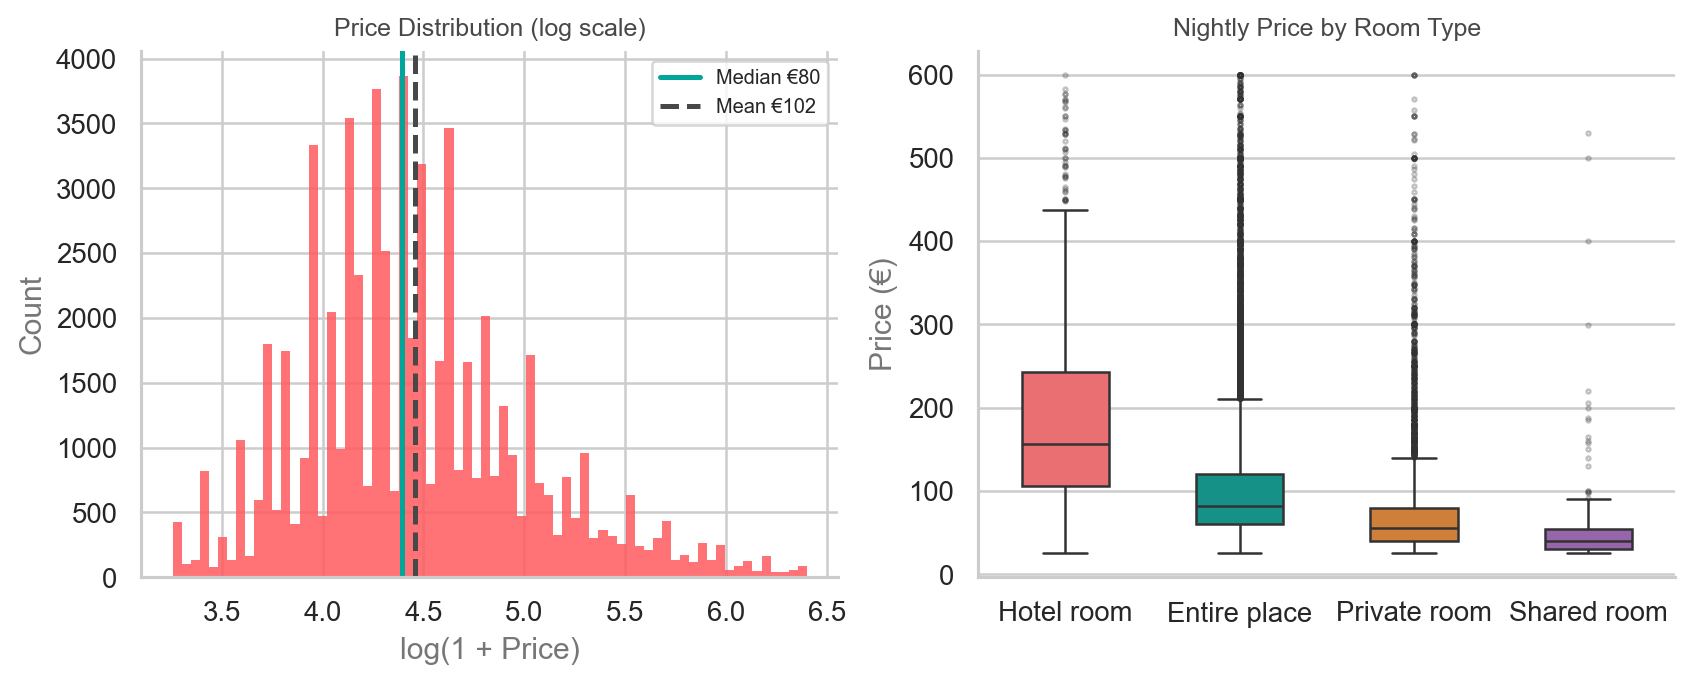
\includegraphics[width=\linewidth]{eda_combined.png}
  \end{columns}
\end{frame}

\begin{frame}{EDA: Geography \& Neighbourhood Pricing}
  \begin{columns}[T]
    \column{0.42\textwidth}
    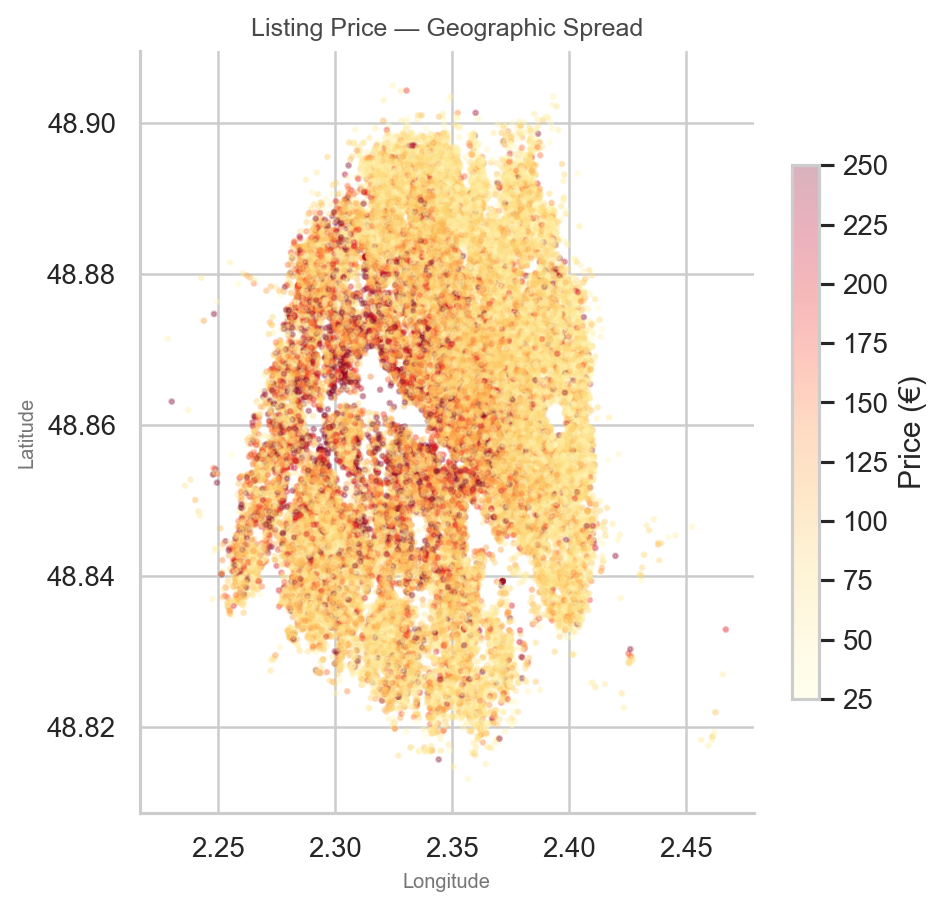
\includegraphics[width=\linewidth]{geo_scatter.png}
    \column{0.56\textwidth}
    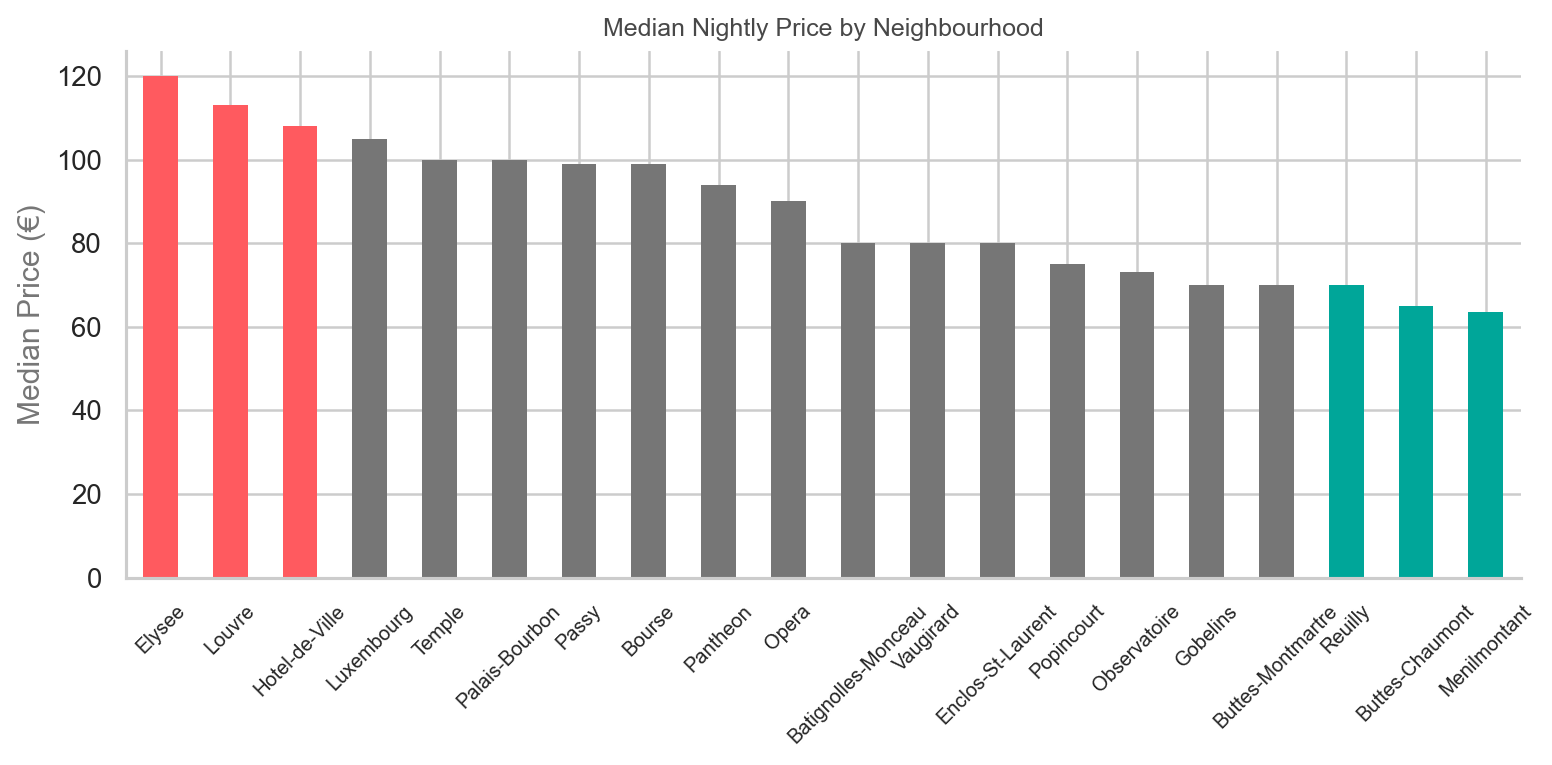
\includegraphics[width=\linewidth]{price_by_neighbourhood.png}
    \vspace{0.1cm}
    \scriptsize\textcolor{airbnbGrey}{
      \hl{Coral}: top-3 most expensive neighbourhoods.
      \tl{Teal}: 3 least expensive.\\
      Geographic scatter confirms price concentration in central Paris.}
  \end{columns}
\end{frame}

\begin{frame}{EDA: Review Activity as a Booking Proxy}
  \begin{columns}[T]
    \column{0.54\textwidth}
    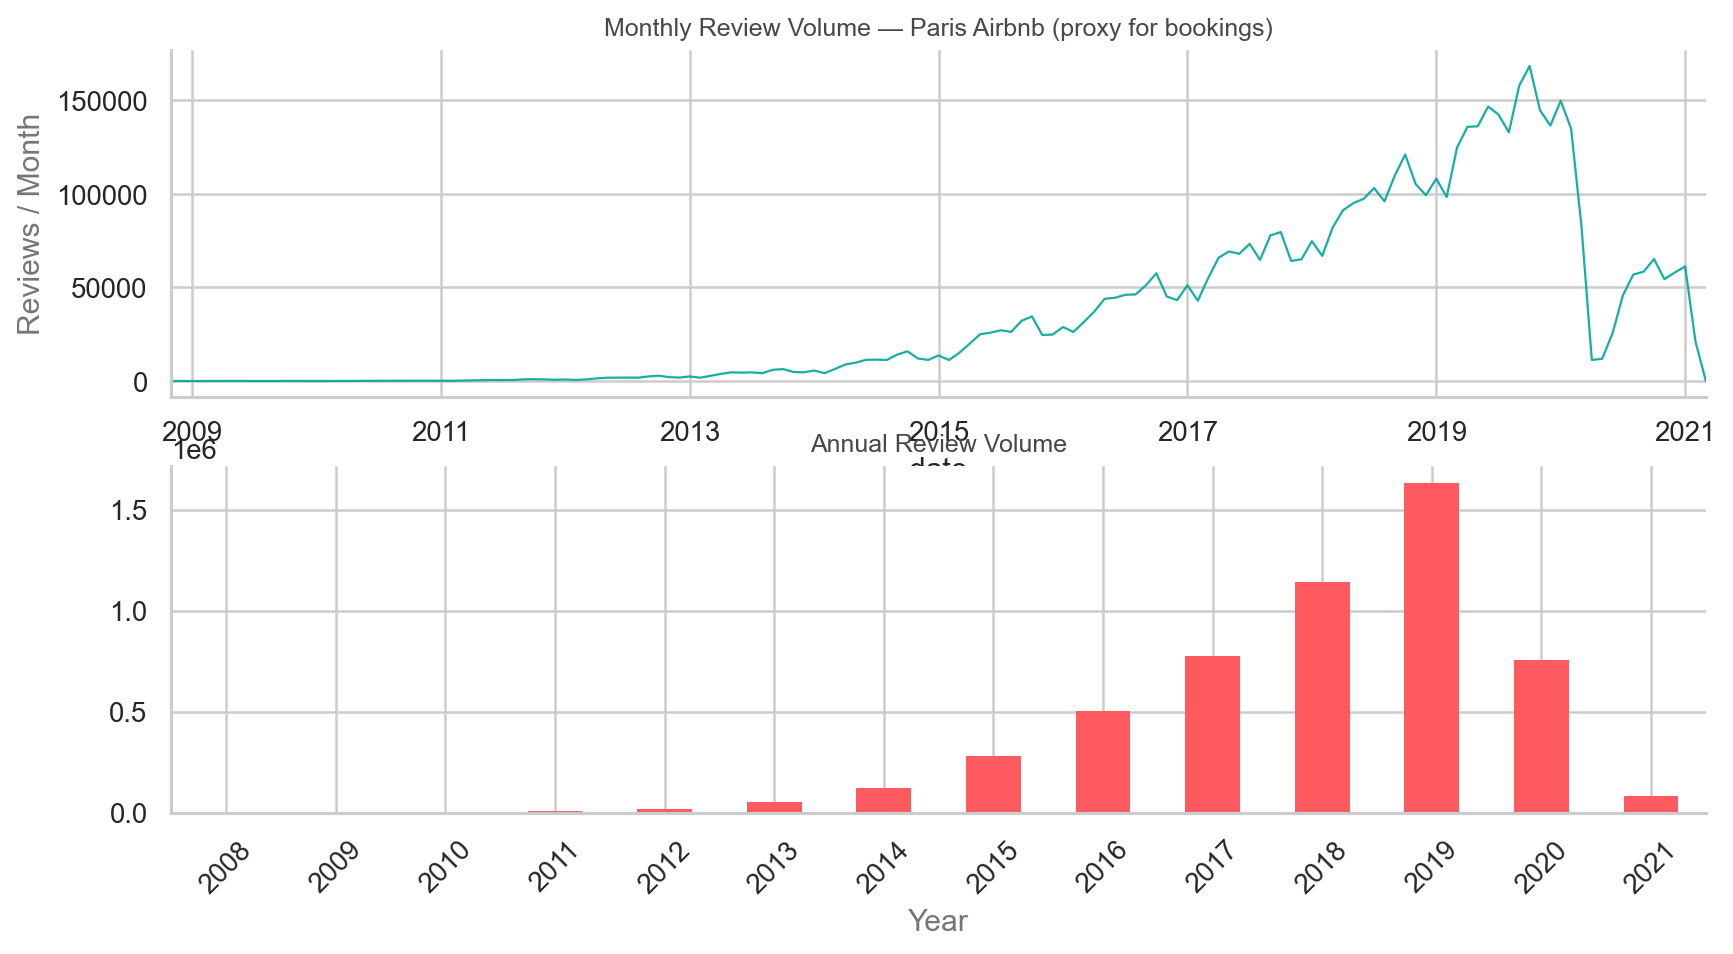
\includegraphics[width=\linewidth]{review_temporal.png}
    \column{0.44\textwidth}
    \small
    \begin{block}{Key observations}
      \begin{itemize}\setlength{\itemsep}{0.3em}
        \item 5.4M reviews across Paris listings
        \item Strong seasonal peaks in summer months
        \item \textbf{COVID-19 dip} clearly visible in 2020--21
        \item Platform growth resumed strongly post-2022
        \item 48\,555 listings have at least 1 review\\(75\% of dataset)
      \end{itemize}
    \end{block}
    \vspace{0.3cm}
    \scriptsize\textcolor{airbnbGrey}{
      Monthly review volume is a reliable proxy for actual bookings
      since only verified stays generate reviews.}
  \end{columns}
\end{frame}

% ============================================================
\section{Feature Engineering \& Selection}
% ============================================================

\begin{frame}[shrink=5]{Feature Engineering: 33 Columns $\rightarrow$ 73 Features}
  \begin{columns}[T]
    \column{0.38\textwidth}
    \scriptsize
    \begin{tabular}{>{\raggedright\arraybackslash}p{1.7cm}
                    >{\raggedright\arraybackslash}p{2.9cm}}
      \toprule
      \textbf{Step} & \textbf{Output}\\
      \midrule
      Outlier filter & p1--p99: \texteuro25--\texteuro600\\[2pt]
      Median impute  & \texttt{bedrooms}, 6 review sub-scores\\[2pt]
      Amenities      & 618 unique $\rightarrow$ 10 binary flags\\[2pt]
      OHE            & \texttt{room\_type}, \texttt{neighbourhood},\\
                     & \texttt{property\_type} (top-10)\\[2pt]
      Distances      & Haversine km to 4 landmarks:\\
                     & Eiffel, Louvre, Notre-Dame,\\
                     & Opera Garnier\\[2pt]
      Review join    & \texttt{review\_count},\\
                     & \texttt{days\_since\_last\_review}\\[2pt]
      Log target     & \texttt{log(1+price)}\\
      \bottomrule
    \end{tabular}
    \vspace{0.2cm}
    {\setbeamerfont{block title}{size=\scriptsize}%
     \setbeamerfont{block body}{size=\scriptsize}%
    \begin{block}{Final feature matrix}
      \textbf{37 features} (union top-30 Lasso + top-20 RF)\\
      on 63\,520 listings
    \end{block}}
    \column{0.60\textwidth}
    \textbf{Feature selection --- 3 methods agree}\\[0.15cm]
    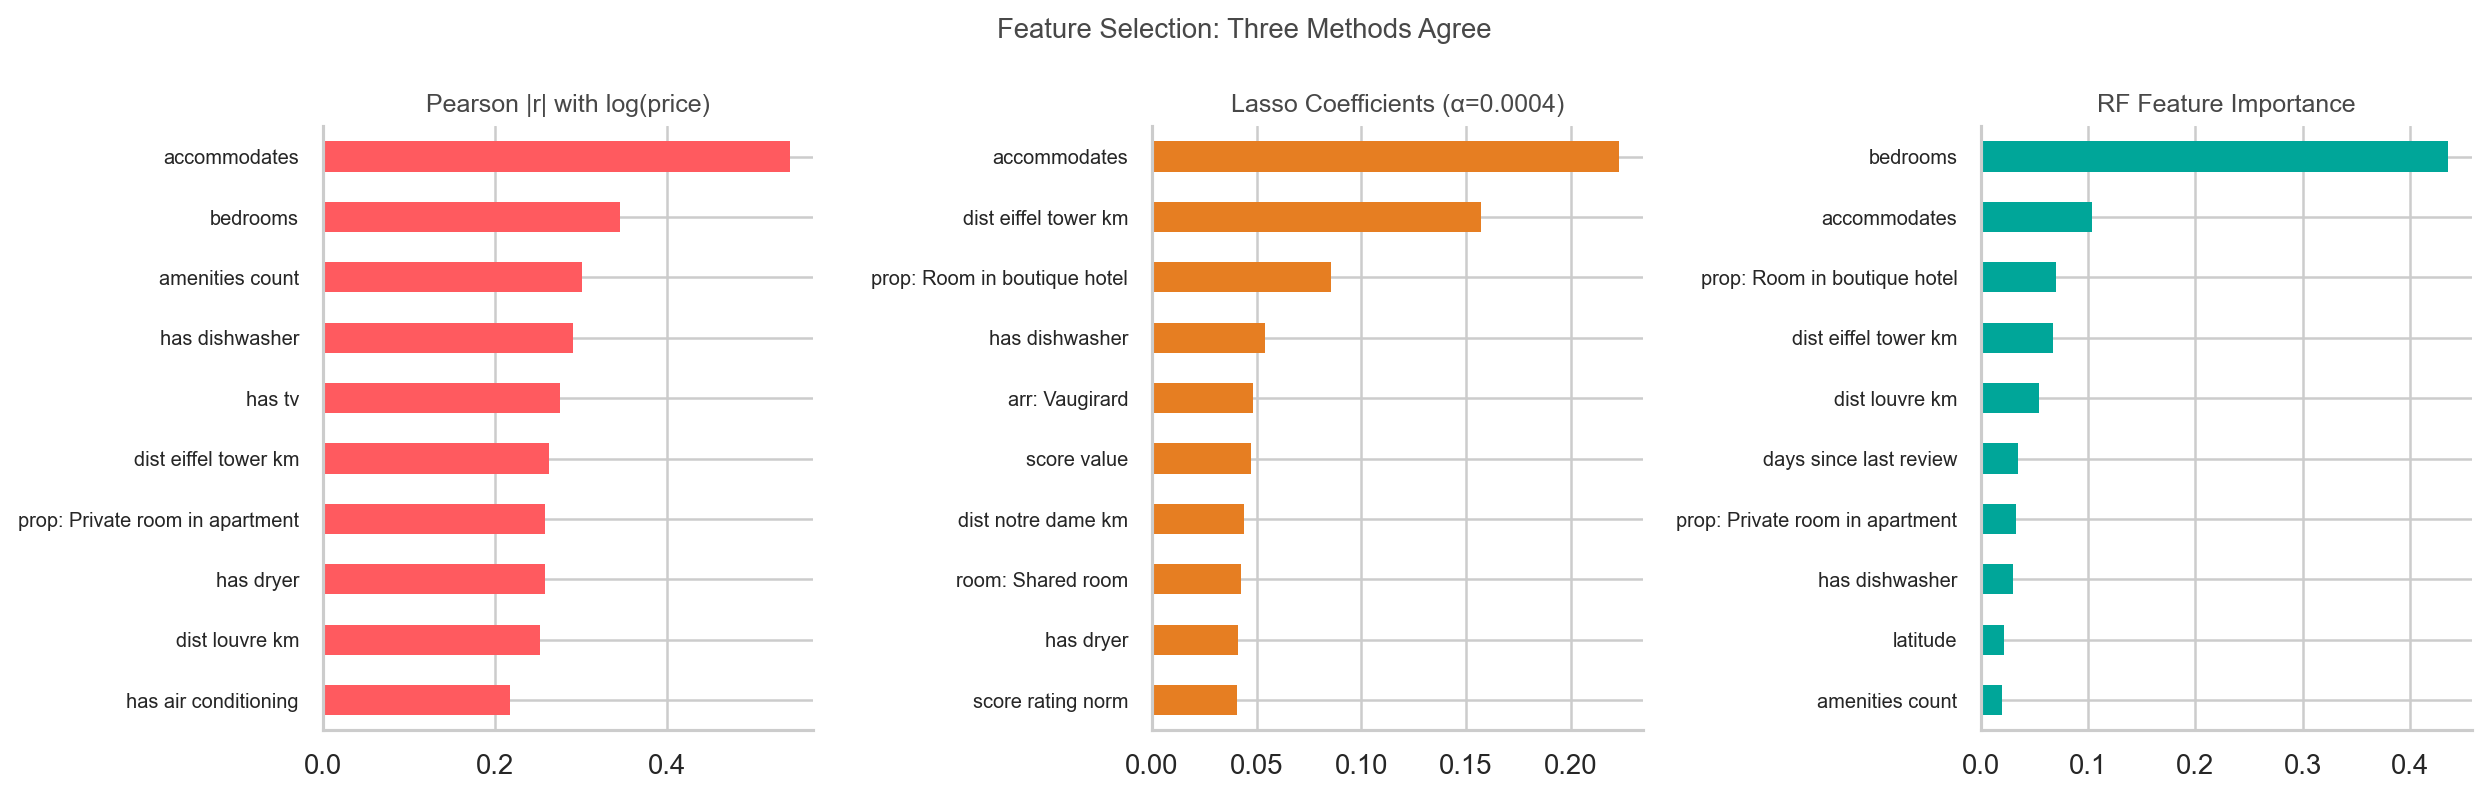
\includegraphics[width=\linewidth]{feature_selection_3panel.png}
    \vspace{0.05cm}
    \scriptsize\textcolor{airbnbGrey}{
      Lasso ($\alpha$=0.0004, 5-fold CV) retains 67/73 features.
      \texttt{bedrooms} dominates RF importance (44\% impurity reduction).
      \texttt{accommodates} leads Pearson ($r$=0.54).}
  \end{columns}
\end{frame}

% ============================================================
\section{Supervised Models}
% ============================================================

\begin{frame}[shrink=10]{All 8 Models --- Performance Comparison}
  \begin{columns}[T]
    \column{0.40\textwidth}
    \scriptsize
    \begin{tabular}{lrrr}
      \toprule
      \textbf{Model} & \textbf{R\textsuperscript{2}} & \textbf{RMSE} & \textbf{MAE}\\
      \midrule
      \rowcolor{airbnbCoral!25}
      Tuned XGBoost   & \textbf{0.658} & \textbf{\texteuro47.2} & \textbf{\texteuro27.2}\\
      Stacking        & 0.651 & \texteuro47.9 & \texteuro27.5\\
      XGBoost         & 0.646 & \texteuro48.5 & \texteuro27.8\\
      MLP Net         & 0.601 & \texteuro50.6 & \texteuro29.6\\
      Random Forest   & 0.600 & \texteuro52.1 & \texteuro29.7\\
      Linear Reg.     & 0.538 & \texteuro56.6 & \texteuro32.5\\
      Ridge           & 0.538 & \texteuro56.6 & \texteuro32.4\\
      Decision Tree   & 0.512 & \texteuro56.0 & \texteuro32.9\\
      \bottomrule
    \end{tabular}
    \vspace{0.25cm}
    \small\textbf{Key takeaways}
    \begin{itemize}\setlength{\itemsep}{0.2em}
      \item XGBoost family \hl{+15 R\textsuperscript{2} pts} vs.\ linear
      \item Stacking (LR+RF+XGB) matches XGBoost
      \item MLP competitive but high CV variance
      \item Average error: \hl{\texteuro27} on \texteuro80 median
    \end{itemize}
    \column{0.58\textwidth}
    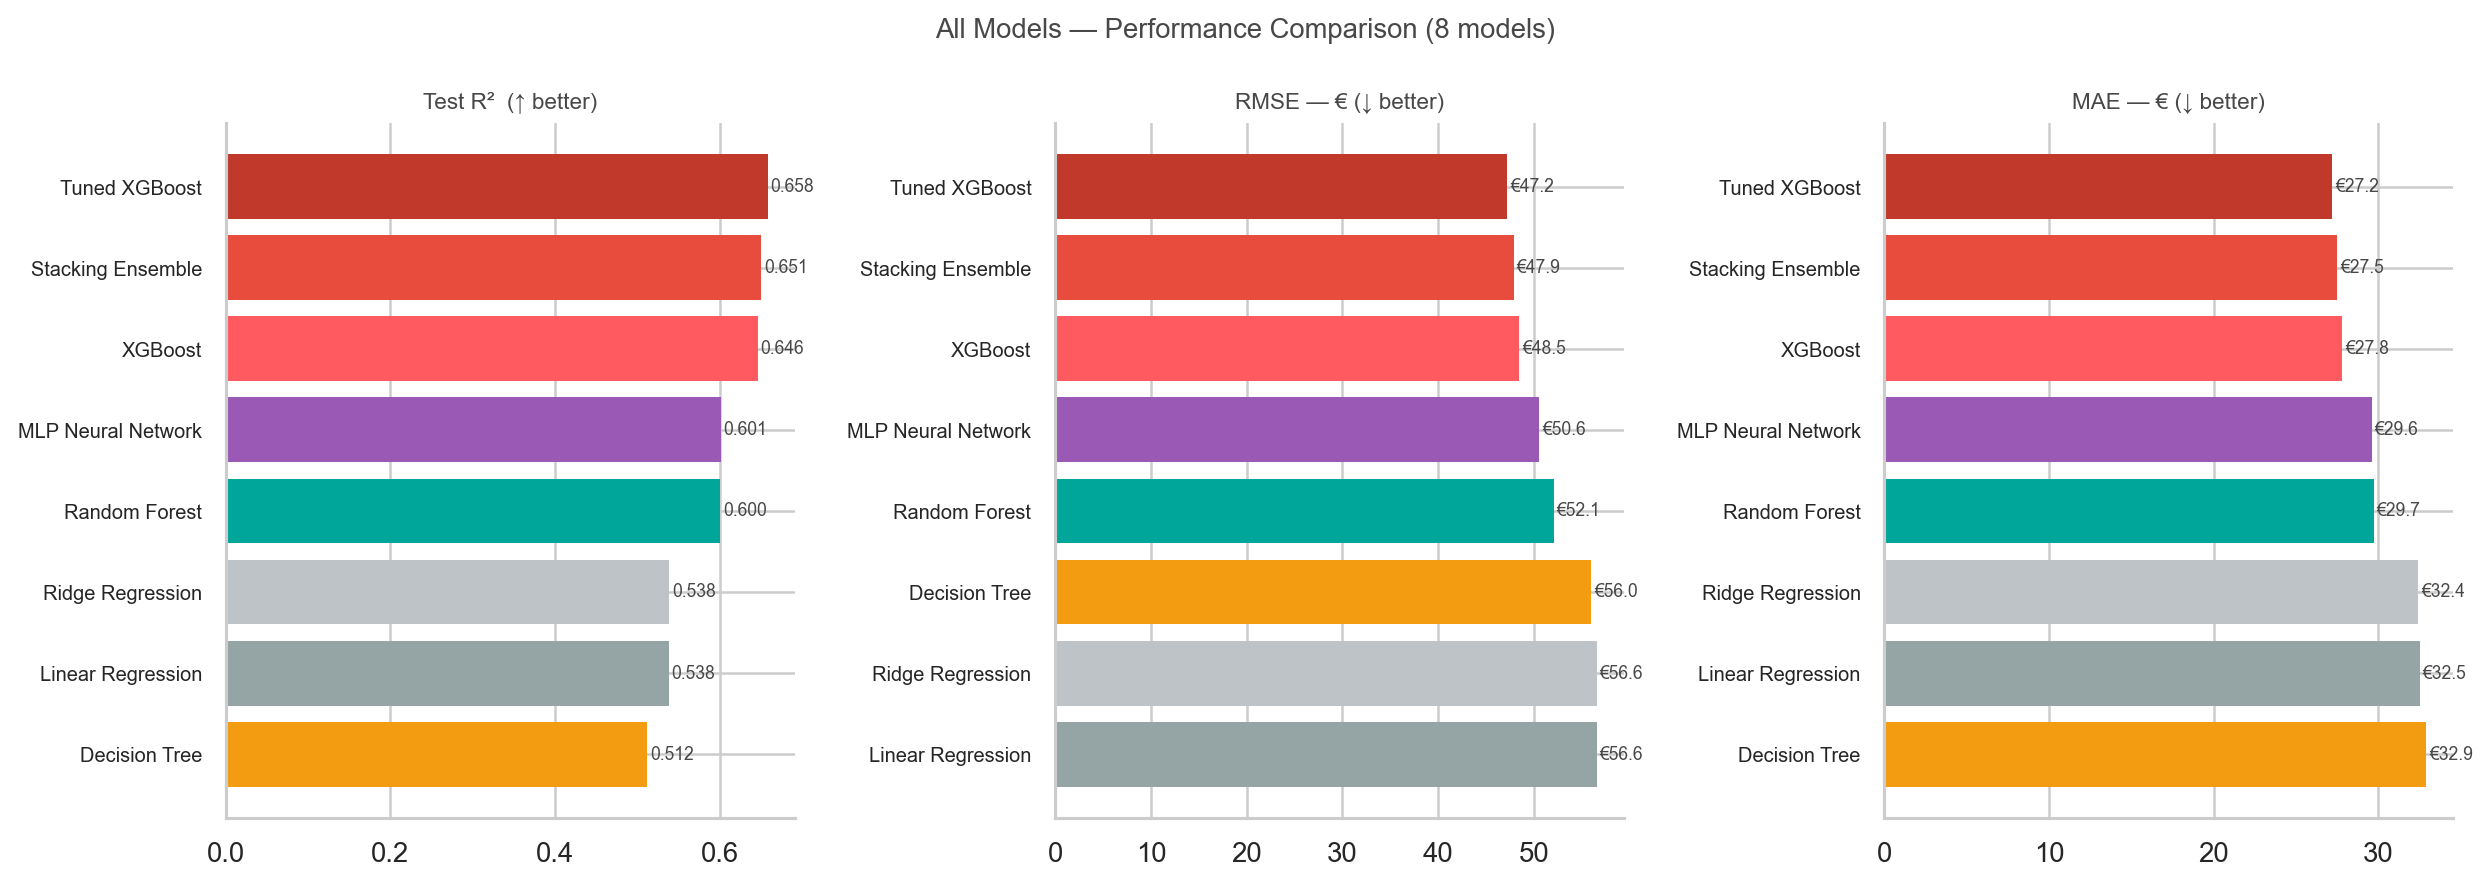
\includegraphics[width=\linewidth, height=0.62\textheight, keepaspectratio]{model_comparison_full.png}
  \end{columns}
\end{frame}

\begin{frame}[shrink=25]{R\textsuperscript{2} with Cross-Validation Uncertainty}
  \begin{columns}[T]
    \column{0.50\textwidth}
    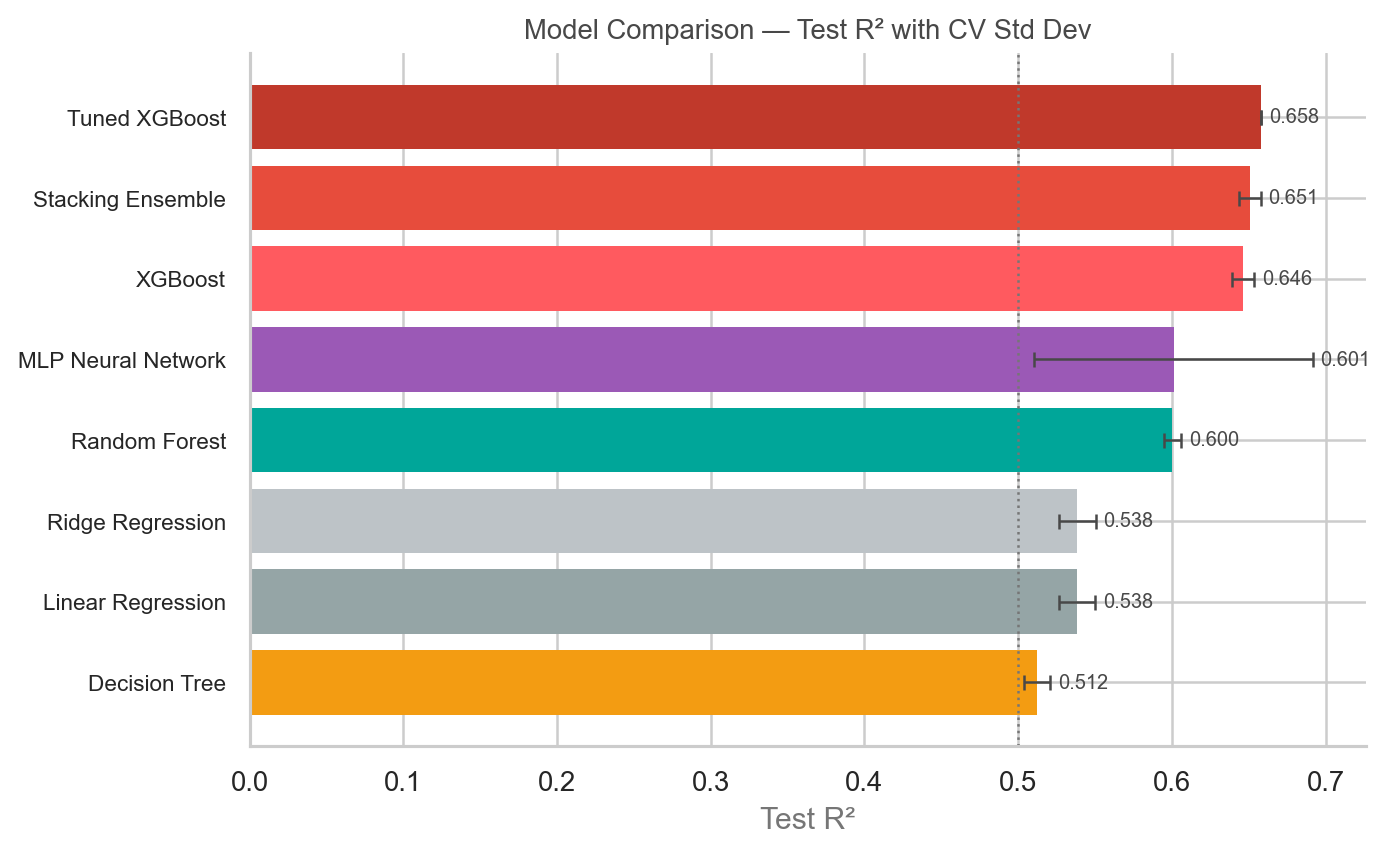
\includegraphics[width=\linewidth]{model_r2_errorbars.png}
    \column{0.48\textwidth}
    \small
    \begin{block}{Reading the chart}
      Error bars show the \textbf{5-fold CV standard deviation}.
      A wide bar means the model is sensitive to which data it trains on.
    \end{block}
    \vspace{0.3cm}
    \textbf{Stability observations}
    \begin{itemize}\setlength{\itemsep}{0.25em}
      \item Linear models: low variance, predictable
      \item \hl{MLP}: high CV std (0.09) --- unstable across folds
      \item XGBoost \& Stacking: \tl{best balance} of performance and stability
      \item Tuned XGBoost (GridSearch): R\textsuperscript{2}=\textbf{0.658}
    \end{itemize}
    \vspace{0.1cm}
    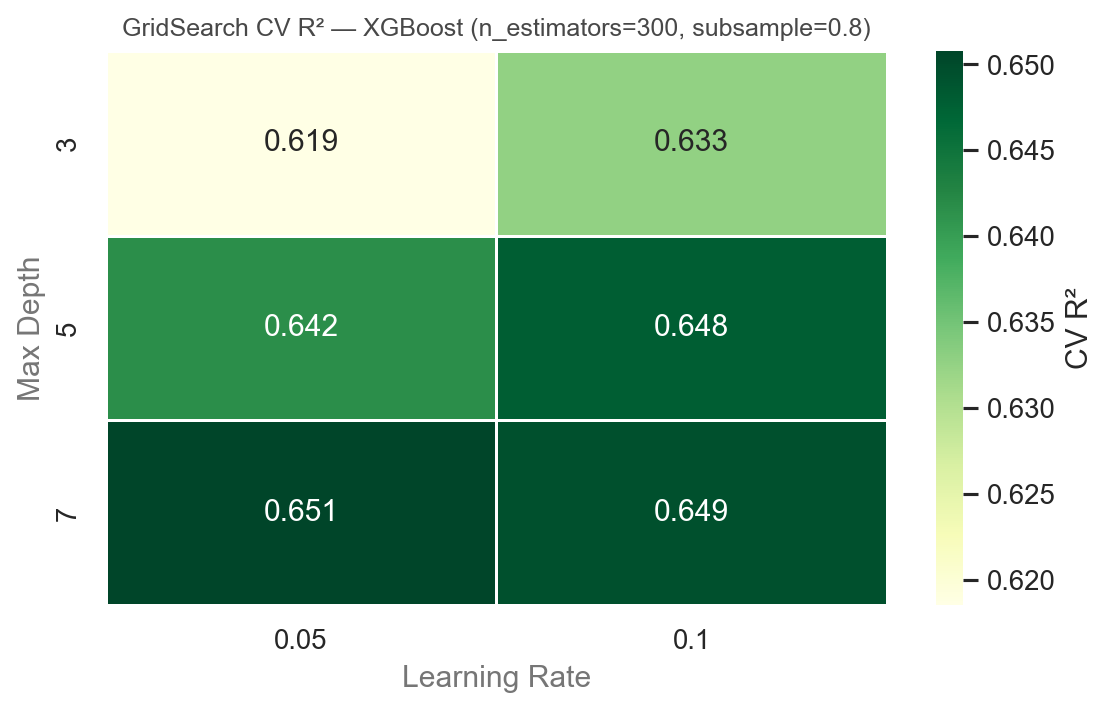
\includegraphics[width=0.7\linewidth]{gridsearch_heatmap.png}
  \end{columns}
\end{frame}

\begin{frame}{XGBoost: Feature Importance \& Residuals}
  \begin{columns}[T]
    \column{0.50\textwidth}
    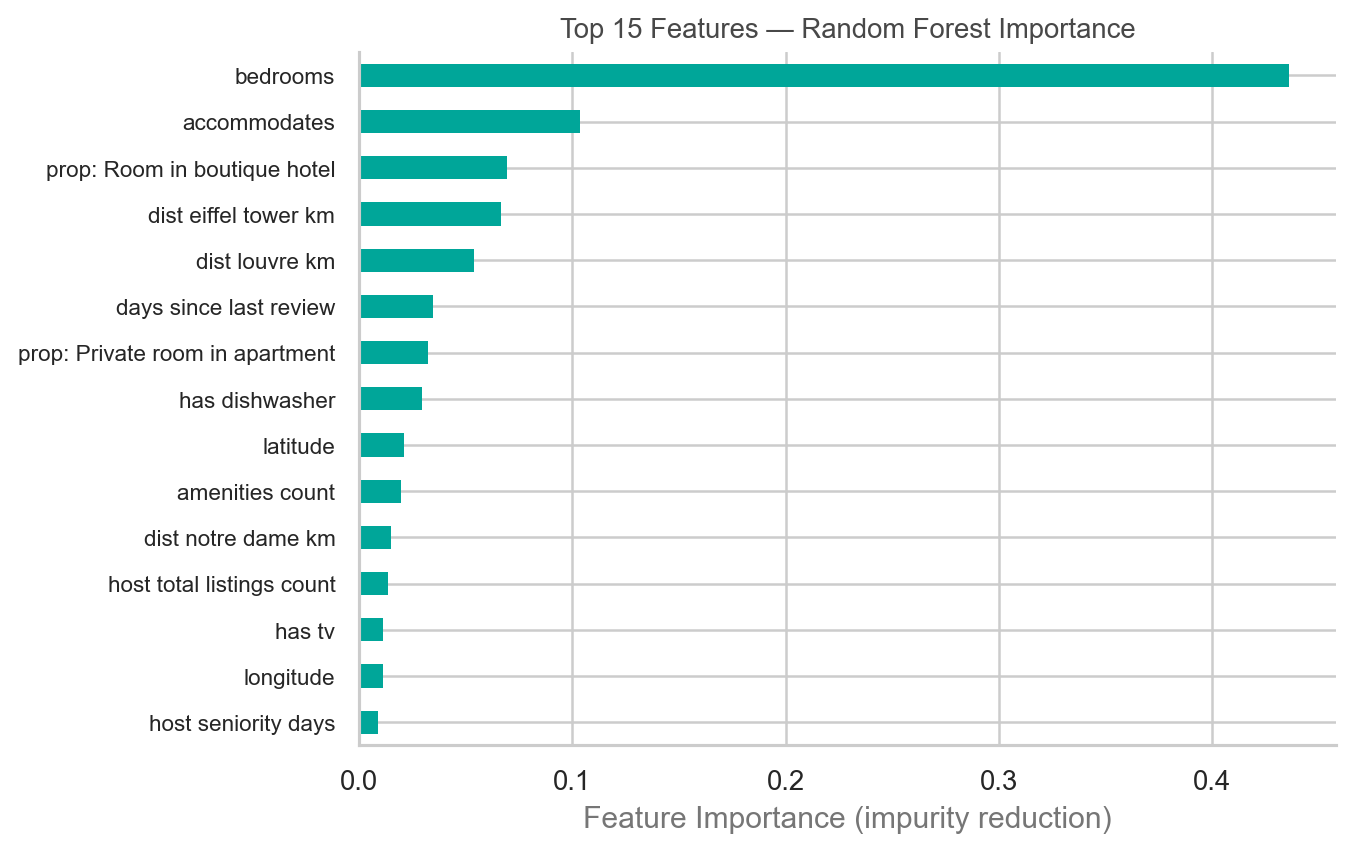
\includegraphics[width=\linewidth]{rf_importance.png}
    \column{0.48\textwidth}
    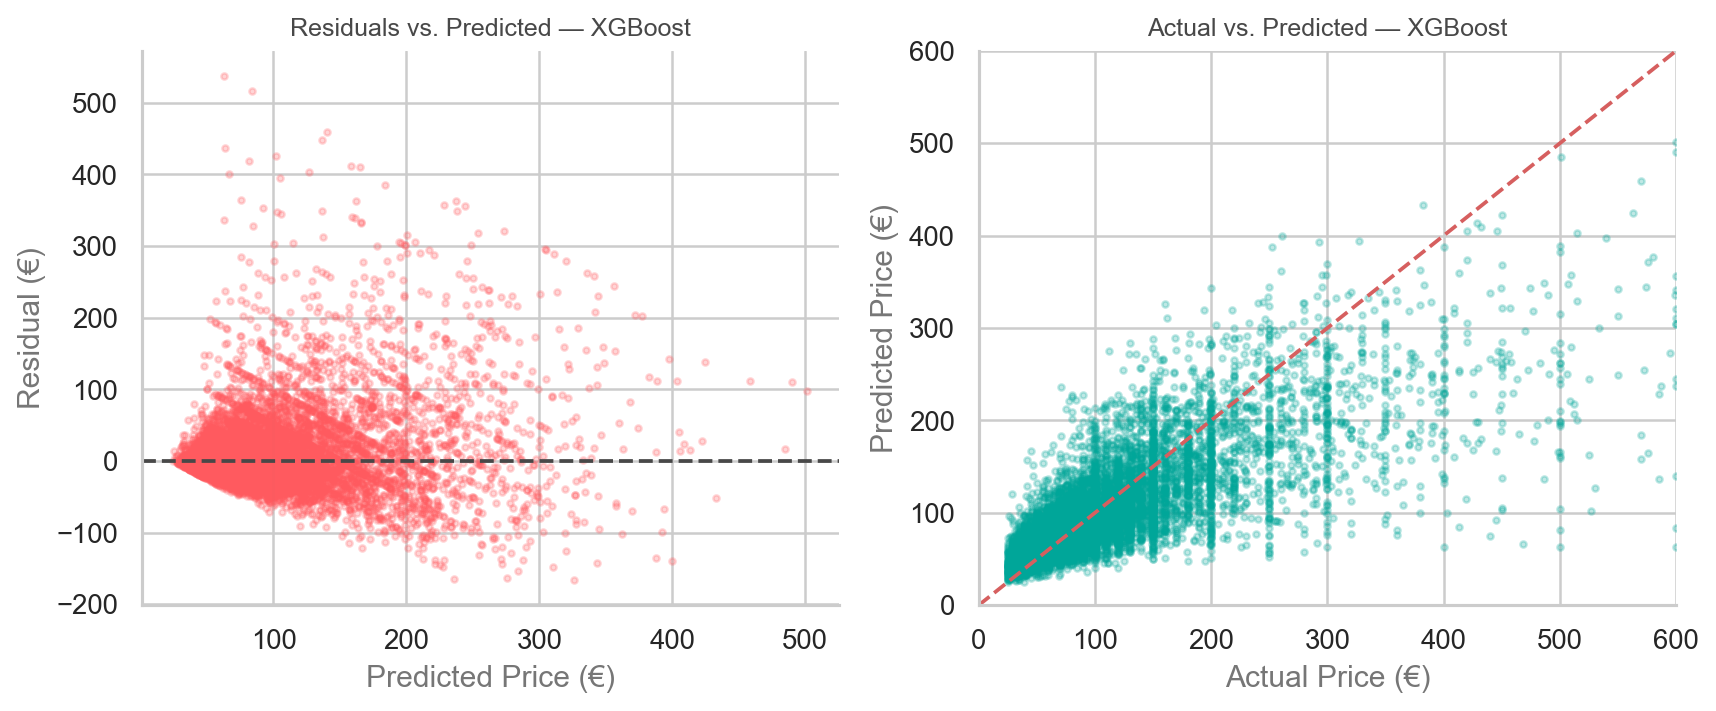
\includegraphics[width=\linewidth]{xgb_residuals.png}
    \vspace{0.15cm}
    \scriptsize\textcolor{airbnbGrey}{
      Residuals centred at zero with no systematic trend ---
      model is unbiased.
      Variance increases for luxury listings ($>$\texteuro400),
      consistent with limited training data at that price level.}
  \end{columns}
\end{frame}

\begin{frame}{MLP Neural Network: Training Dynamics}
  \begin{columns}[T]
    \column{0.55\textwidth}
    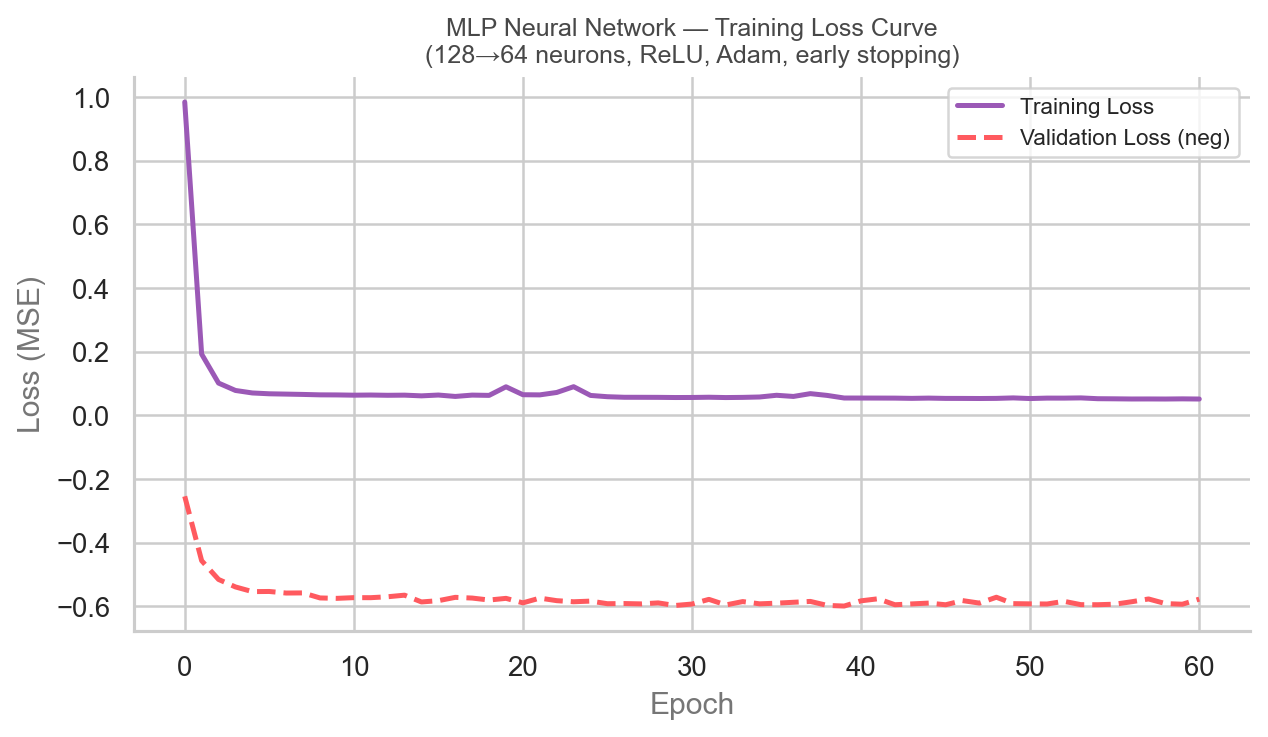
\includegraphics[width=\linewidth]{mlp_loss_curve.png}
    \column{0.43\textwidth}
    \small\textbf{Architecture}
    \begin{itemize}\setlength{\itemsep}{0.25em}
      \item Two hidden layers: \textbf{128 $\rightarrow$ 64} neurons
      \item Activation: ReLU
      \item Optimiser: Adam
      \item Early stopping (patience = 20 epochs)
      \item Validation split: 10\,\%
    \end{itemize}
    \vspace{0.3cm}
    \begin{block}{Results}
      \small
      Test R\textsuperscript{2}: \textbf{0.601} $\cdot$ RMSE: \texteuro50.6\\
      CV R\textsuperscript{2}: 0.544 $\pm$ 0.09\\
      \textit{Competitive but less stable than XGBoost}
    \end{block}
  \end{columns}
\end{frame}

% ============================================================
\section{Classification: Price Tiers}
% ============================================================

\begin{frame}{Price Tier Classification: 3 Classifiers Compared}
  \begin{columns}[T]
    \column{0.62\textwidth}
    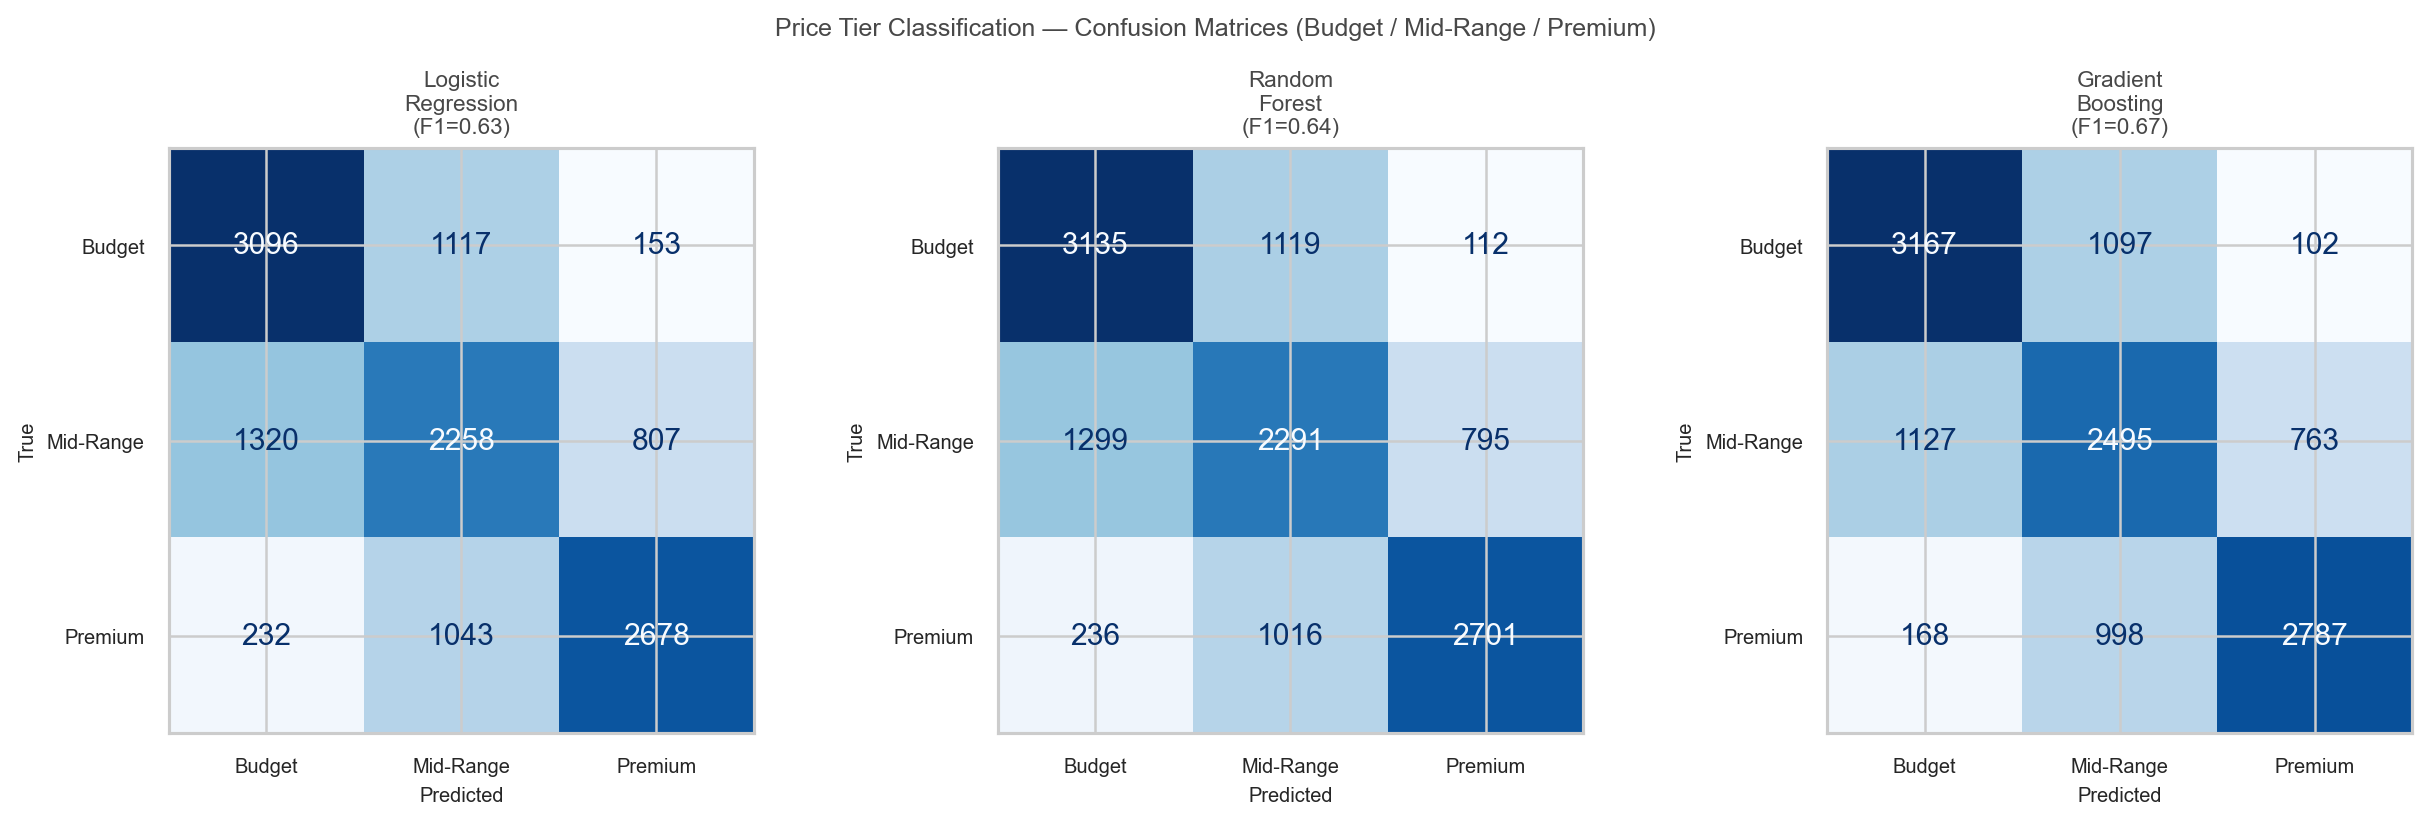
\includegraphics[width=\linewidth]{classification_confusion.png}
    \column{0.36\textwidth}
    \small\textbf{Task}\\
    3 balanced tiers via quantile cut:
    \begin{itemize}\setlength{\itemsep}{0.15em}
      \item Budget ($<$\texteuro66)
      \item Mid-Range (\texteuro66--\texteuro110)
      \item Premium ($>$\texteuro110)
    \end{itemize}
    \vspace{0.3cm}
    \textbf{F1 scores}
    \begin{itemize}\setlength{\itemsep}{0.15em}
      \item Logistic Reg.: \textbf{0.63}
      \item Random Forest: strong
      \item \hl{Gradient Boosting}: best
    \end{itemize}
    \vspace{0.3cm}
    \scriptsize\textcolor{airbnbGrey}{
      Mid-Range is hardest to classify --- boundary effects
      between tiers. Premium and Budget are most distinct.}
  \end{columns}
\end{frame}

% ============================================================
\section{Amenity Analysis}
% ============================================================

\begin{frame}[shrink=3]{Amenity Analysis: Which Amenities Add Value?}
  \begin{columns}[T]
    \column{0.54\textwidth}
    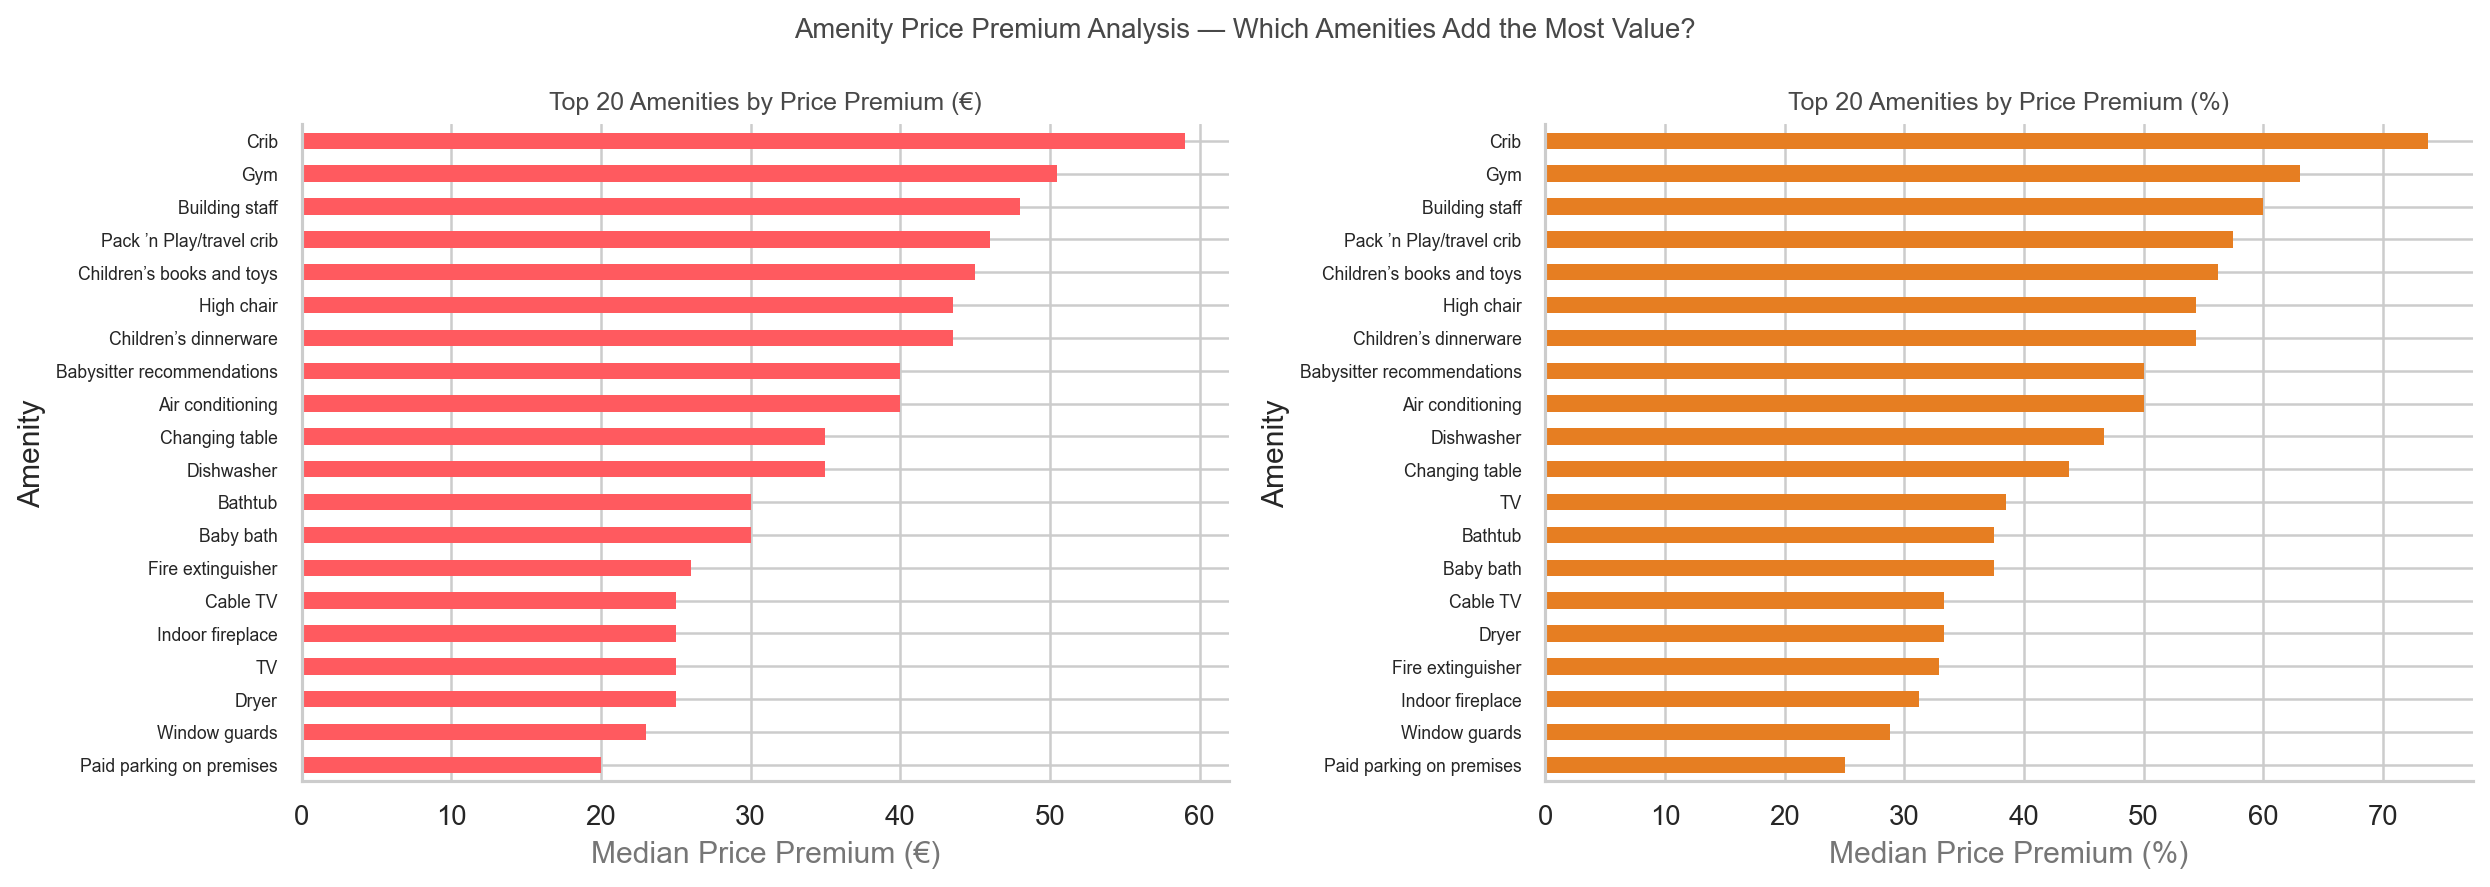
\includegraphics[width=\linewidth]{amenity_premium.png}
    \column{0.44\textwidth}
    \small
    \begin{block}{Methodology}
      For each of 76 amenities (present in $\geq$500 listings):
      compare median price \textbf{with} vs.\ \textbf{without}
      that amenity.
    \end{block}
    \vspace{0.2cm}
    \textbf{Top value-add amenities}
    \begin{itemize}\setlength{\itemsep}{0.2em}
      \item Pool, hot tub, sauna: highest absolute premium
      \item Elevator, A/C, dishwasher: strong per-\texteuro uplift
      \item Wifi \& Kitchen: near-universal --- little marginal gain
    \end{itemize}
    \vspace{0.1cm}
    {\setbeamerfont{block title}{size=\footnotesize}%
     \setbeamerfont{block body}{size=\footnotesize}%
    \begin{block}{Actionable insight}
      Adding amenities with high premium \% to your listing
      can justify a meaningful price increase.
    \end{block}}
  \end{columns}
\end{frame}

\begin{frame}[shrink=5]{Amenity Decision Tree --- Price Tier Prediction}
  \begin{center}
    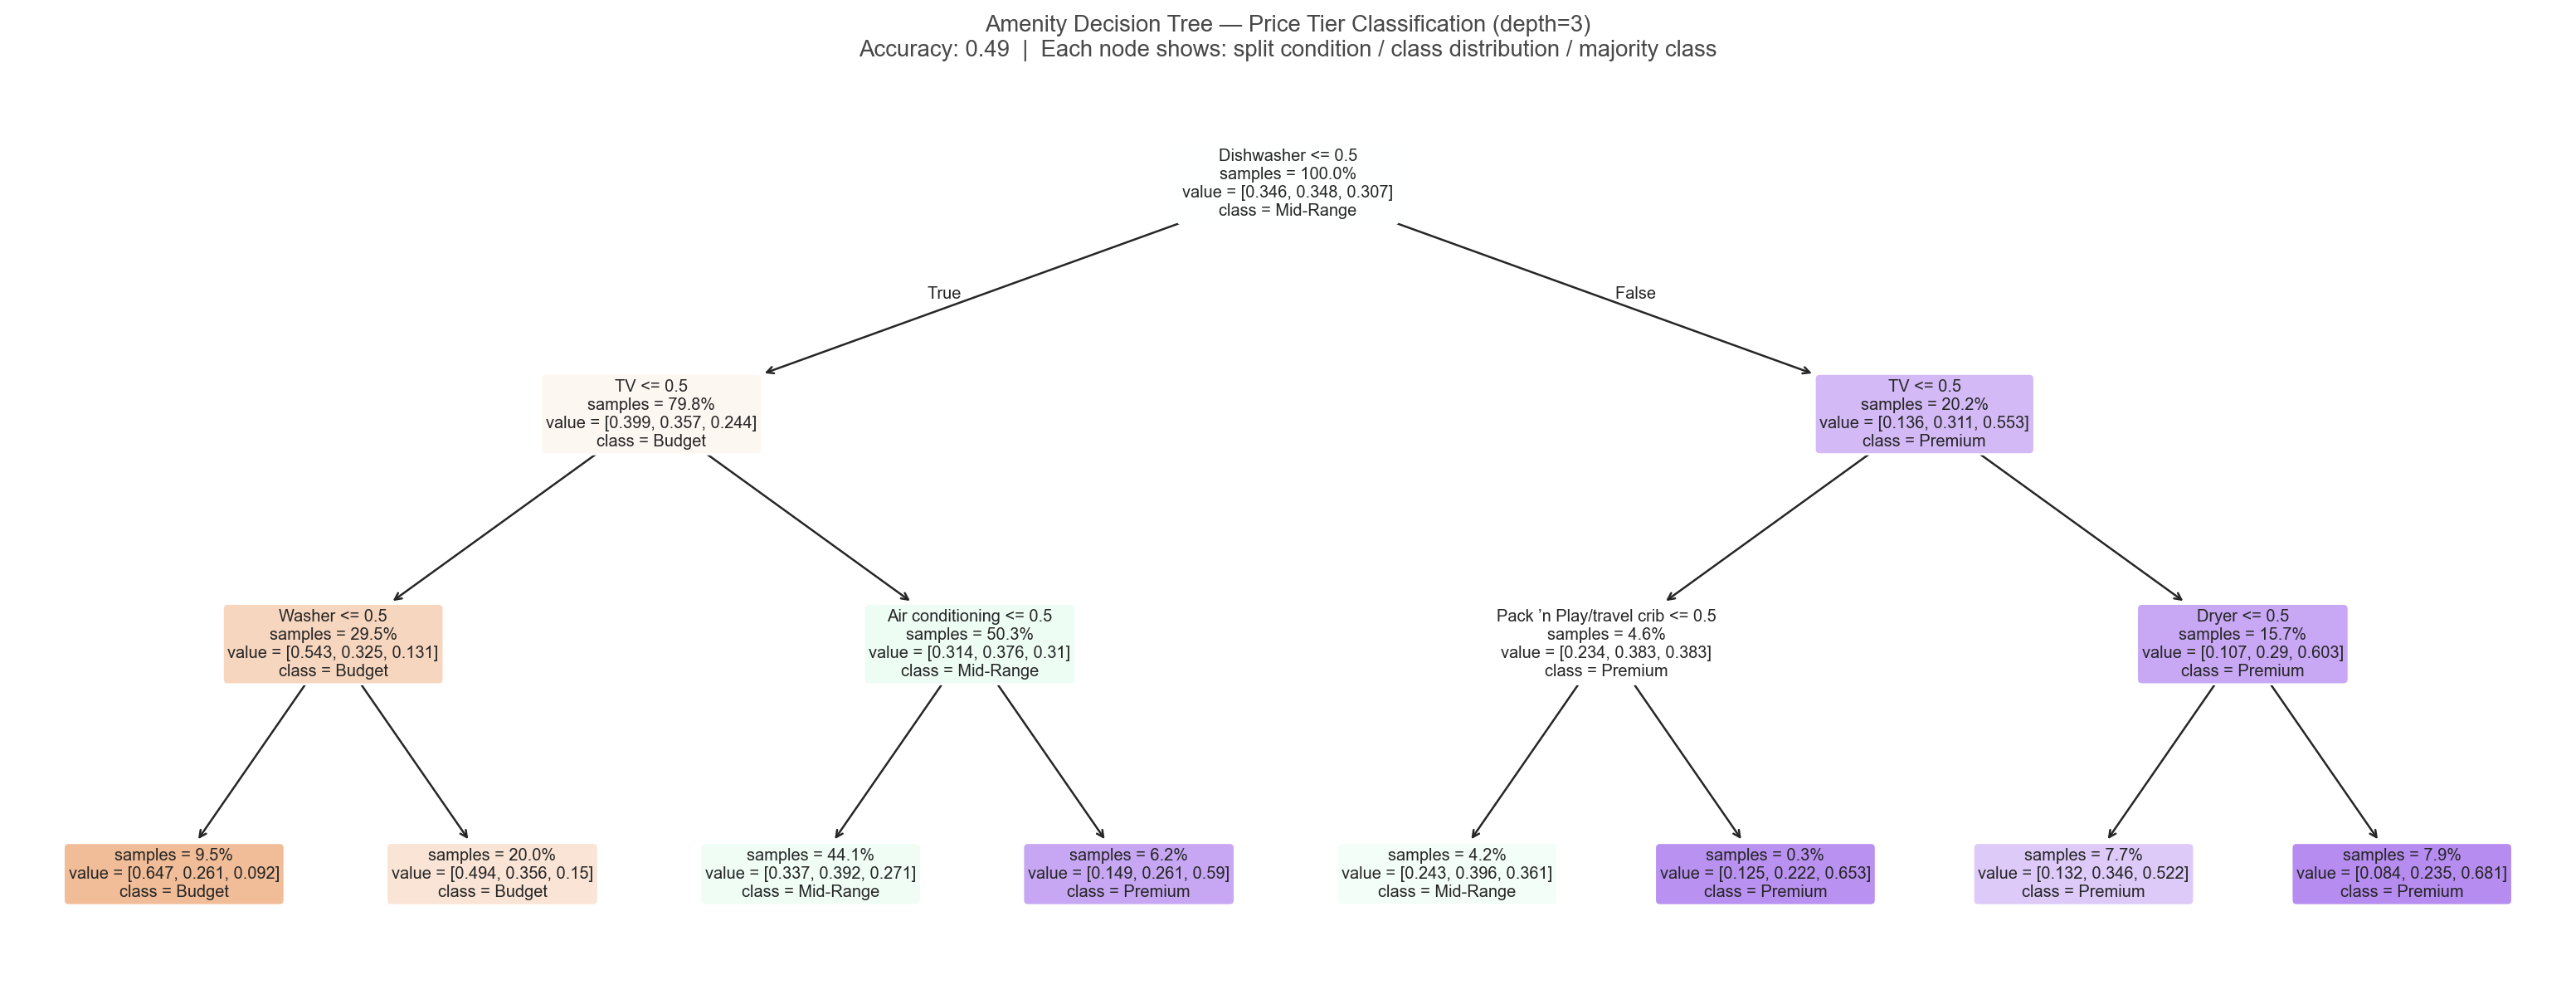
\includegraphics[width=0.97\linewidth]{amenity_decision_tree.png}
  \end{center}
  \vspace{-0.2cm}
  \parbox{\linewidth}{\scriptsize\textcolor{airbnbGrey}{%
    Decision tree (depth=3) trained on 76 binary amenity features only.
    Accuracy: 0.49 --- amenities alone explain $\approx$23\% of price variance.
    Location and capacity explain the remainder.
    Tree shows which amenity combinations most distinguish Budget from Premium listings.}}
\end{frame}

% ============================================================
\section{Listing Segmentation}
% ============================================================

\begin{frame}[shrink=8]{K-Means Clustering: Selecting k = 4}
  \begin{columns}[T]
    \column{0.55\textwidth}
    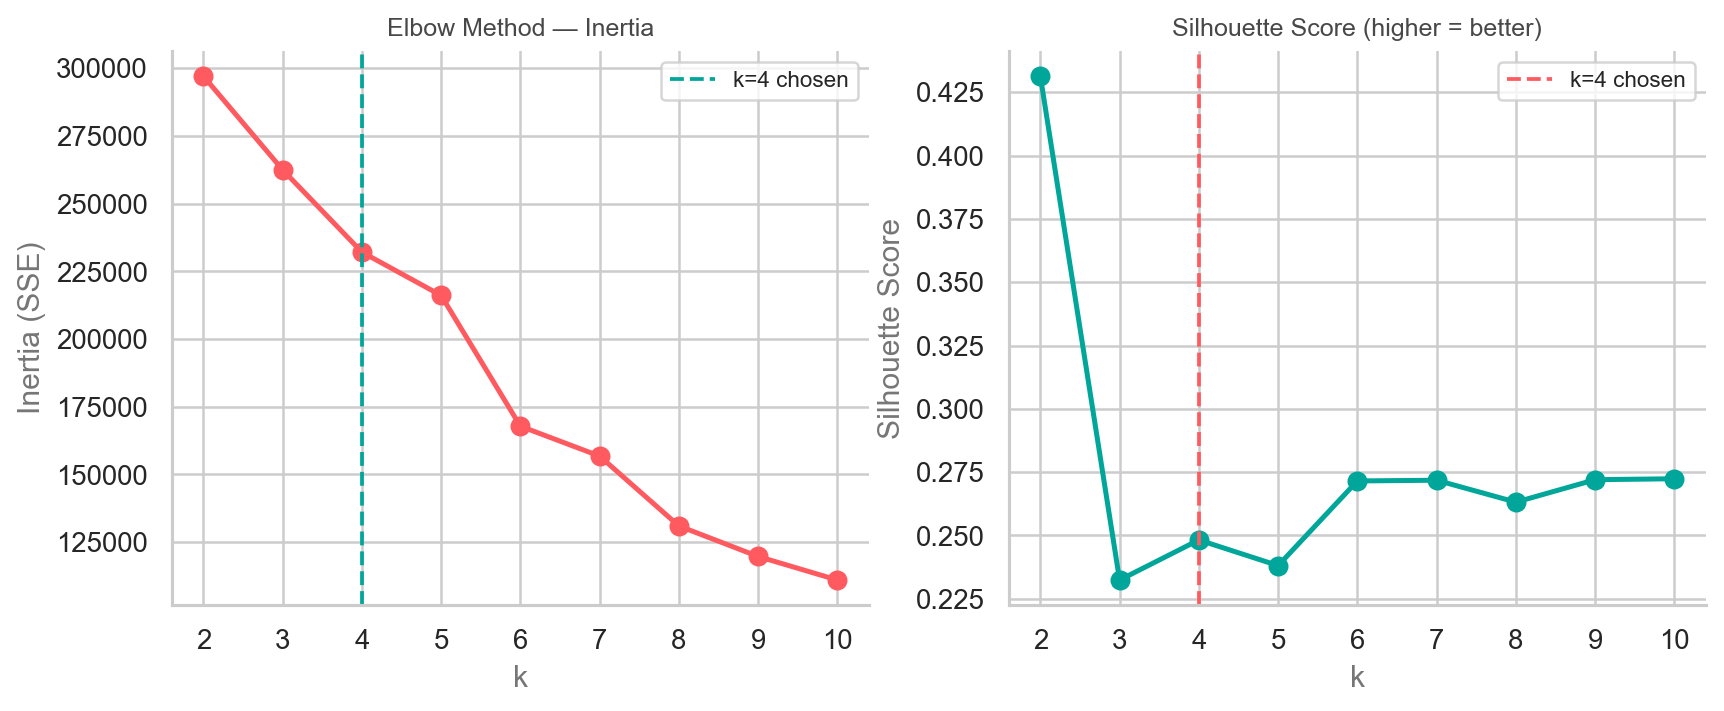
\includegraphics[width=\linewidth]{elbow_silhouette.png}
    \vspace{0.1cm}
    \parbox{\linewidth}{\scriptsize\textcolor{airbnbGrey}{%
      Elbow: inertia flattens after k=4.
      Silhouette peaks at k=2 but k=4 gives the best interpretable segmentation.
      Hierarchical clustering (Ward) agrees at \textbf{78\,\%}.}}
    \column{0.43\textwidth}
    \small\textbf{Clustering features}
    \begin{itemize}\setlength{\itemsep}{0.2em}
      \item \texttt{accommodates}, \texttt{bedrooms}
      \item \texttt{amenities\_count}
      \item Overall rating (normalised)
      \item Host listing count (capped)
      \item \texttt{price}
    \end{itemize}
    \vspace{0.25cm}
    \scriptsize
    \begin{tabular}{>{\bfseries}lrrr}
      \toprule
      Segment & n & Guests & \texteuro\\
      \midrule
      \textcolor{clusterRed}{Spacious}   & 8\,017 & 5.3 & \textbf{214}\\
      \textcolor{clusterBlue}{Mid-Range} & 19\,694 & 2.5 & 94\\
      \textcolor{clusterGreen}{Standard} & 31\,045 & 2.0 & 76\\
      \textcolor{clusterOrange}{Budget}  & 4\,731 & 1.6 & 59\\
      \bottomrule
    \end{tabular}
  \end{columns}
\end{frame}

\begin{frame}[shrink=5]{Cluster Profiles \& Dendrogram Validation}
  \begin{columns}[T]
    \column{0.52\textwidth}
    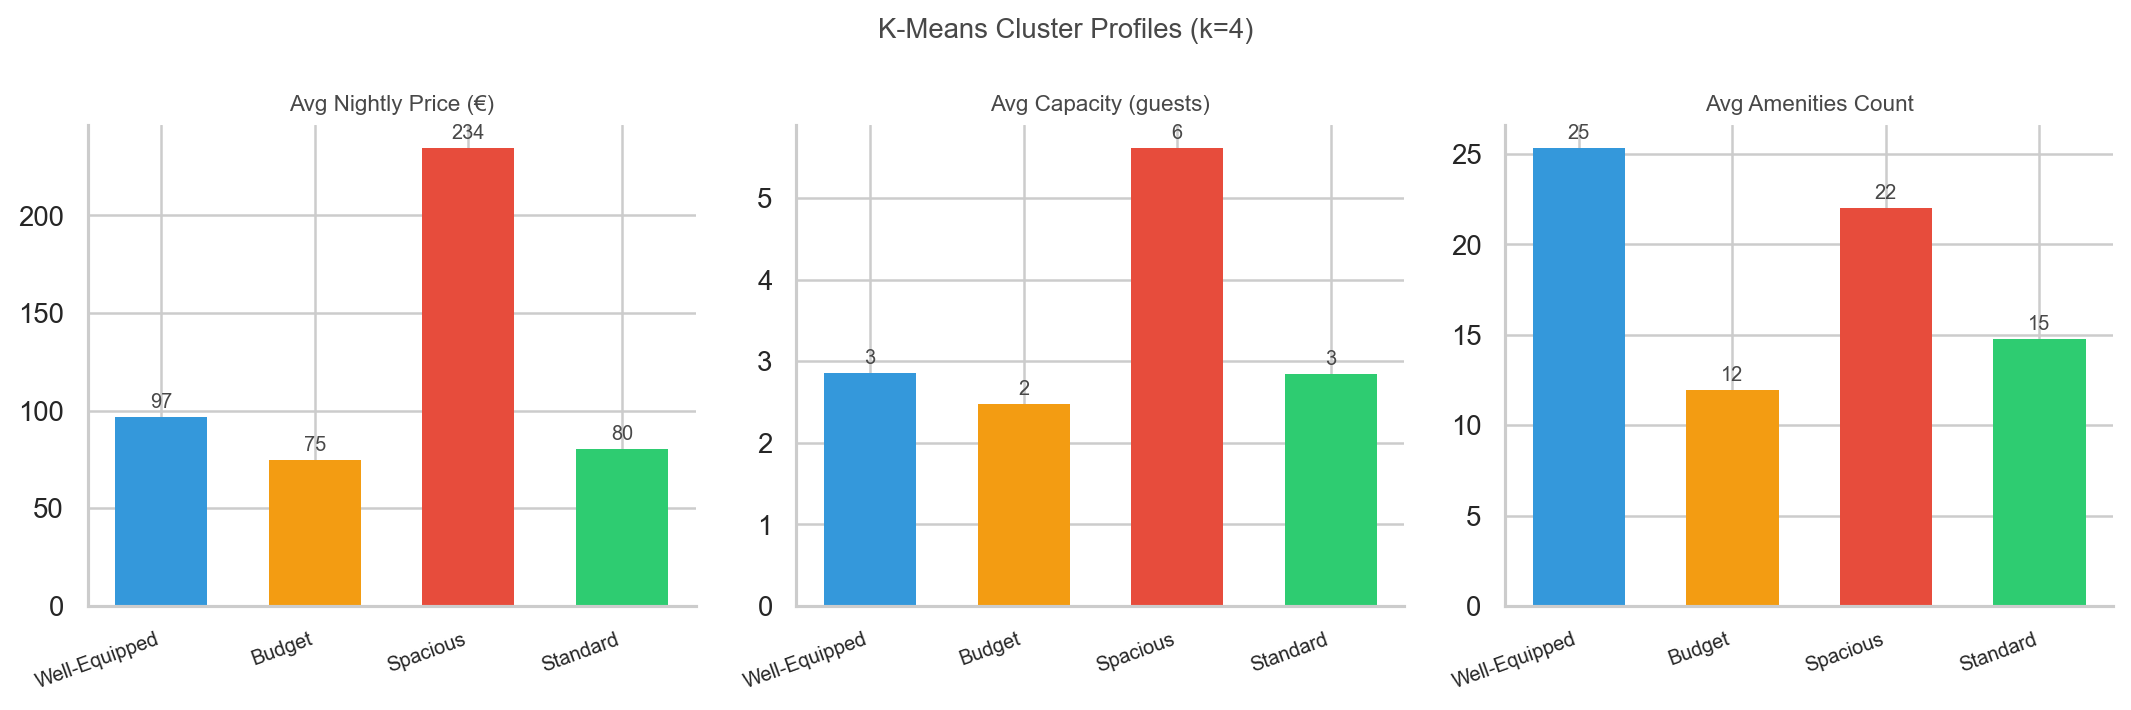
\includegraphics[width=\linewidth]{cluster_profiles.png}
    \vspace{0.05cm}
    \parbox{\linewidth}{\scriptsize\textcolor{airbnbGrey}{%
      \textcolor{clusterRed}{$\blacksquare$}~\textbf{Spacious \& Premium}: large, expensive.
      \textcolor{clusterBlue}{$\blacksquare$}~\textbf{Mid-Range}: solid amenity set.\\
      \textcolor{clusterGreen}{$\blacksquare$}~\textbf{Standard Compact}: most common ($\approx$50\%).
      \textcolor{clusterOrange}{$\blacksquare$}~\textbf{Budget Basic}: smallest.}}
    \column{0.46\textwidth}
    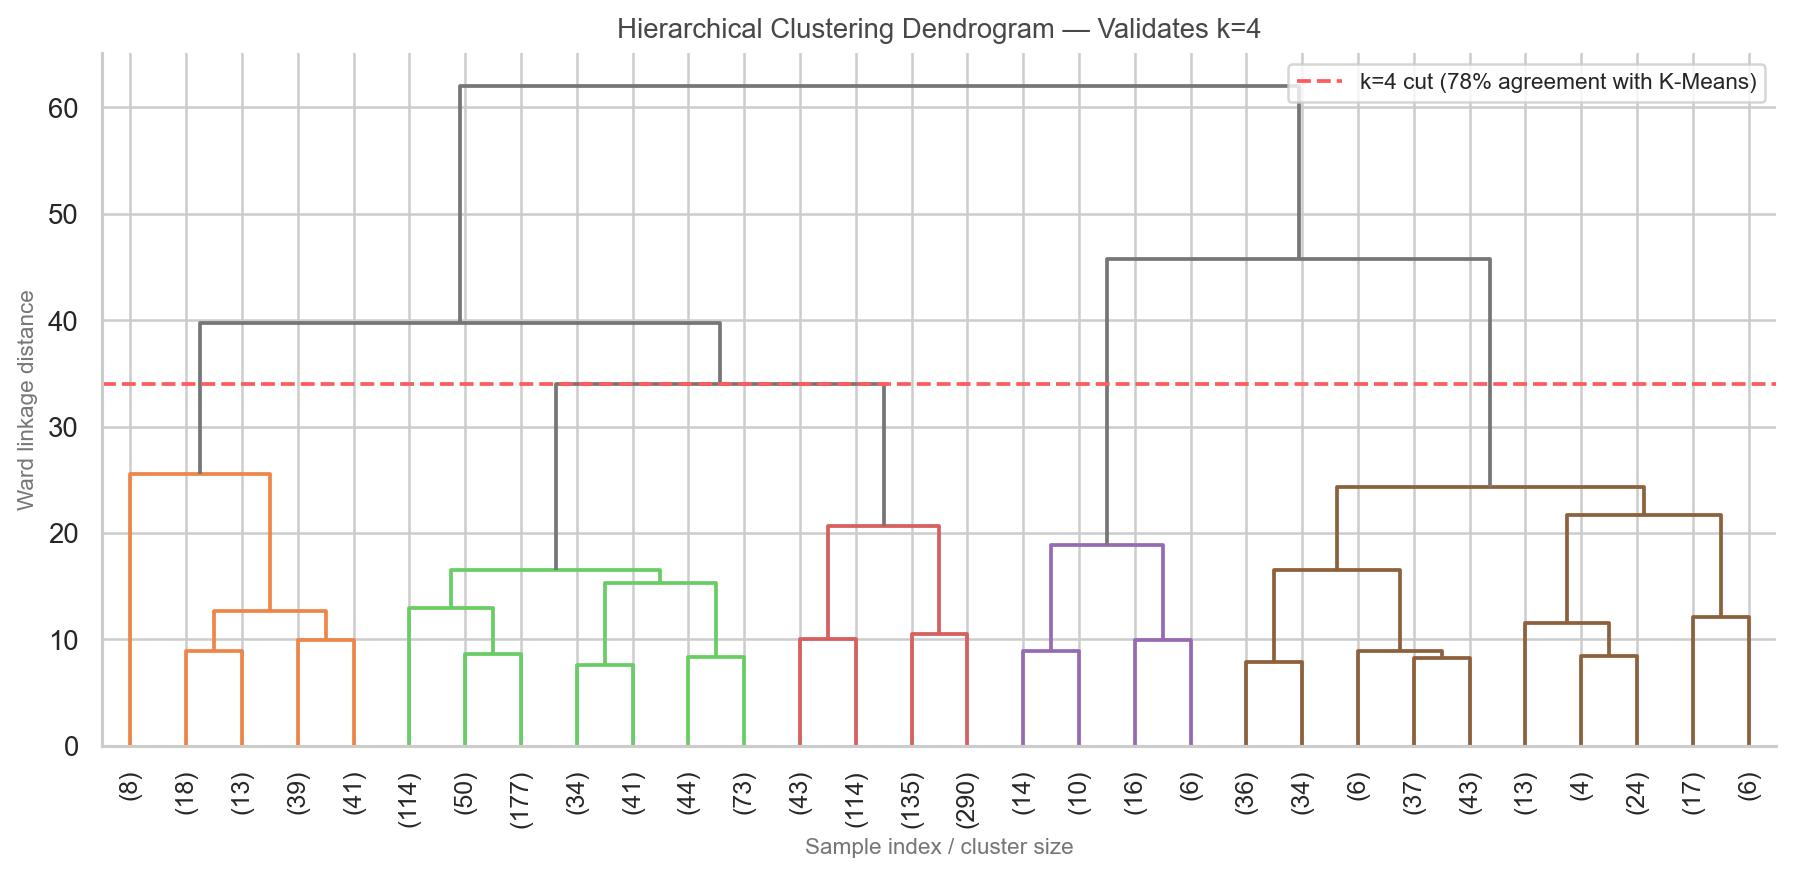
\includegraphics[width=\linewidth]{dendrogram.png}
    \vspace{0.05cm}
    \parbox{\linewidth}{\scriptsize\textcolor{airbnbGrey}{%
      Ward dendrogram (1\,500-listing sample).
      Red dashed line = k=4 cut.
      78\% agreement with K-Means.}}
  \end{columns}
\end{frame}

\begin{frame}[shrink=5]{Cluster Visualisation: PCA \& t-SNE}
  \begin{columns}[T]
    \column{0.50\textwidth}
    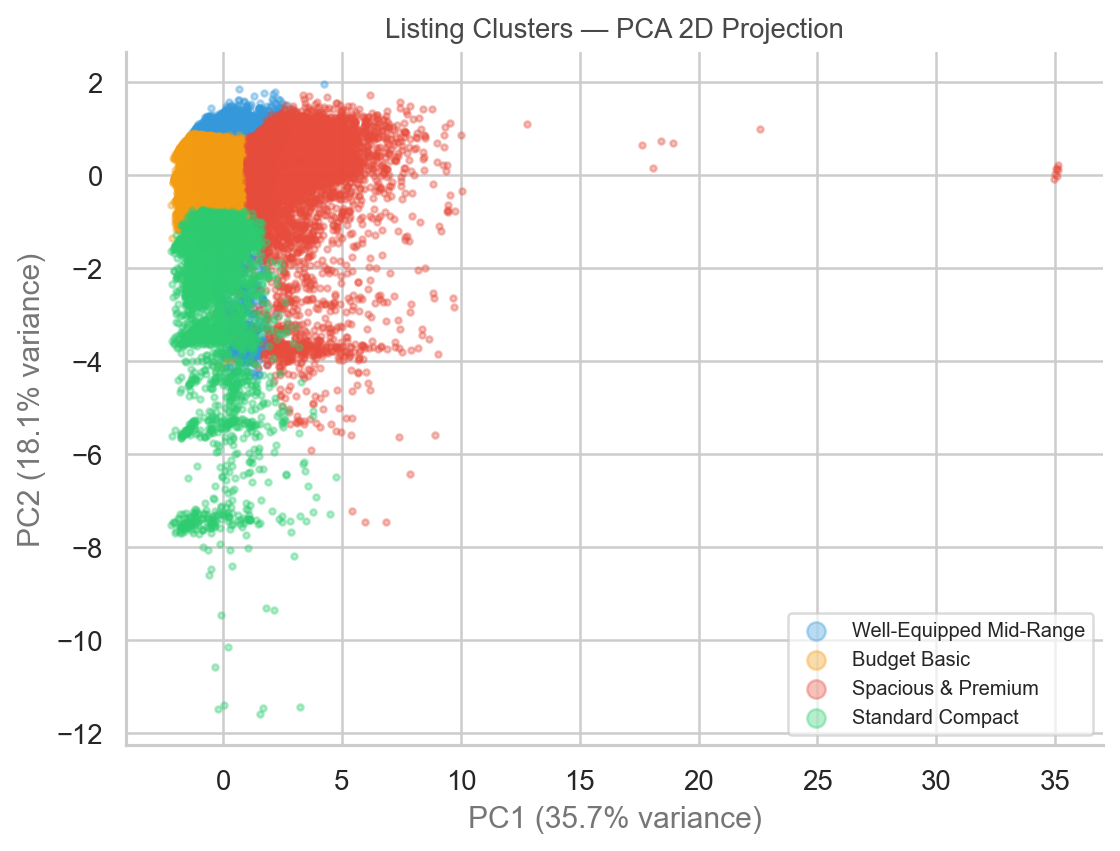
\includegraphics[width=\linewidth]{cluster_pca.png}
    \column{0.48\textwidth}
    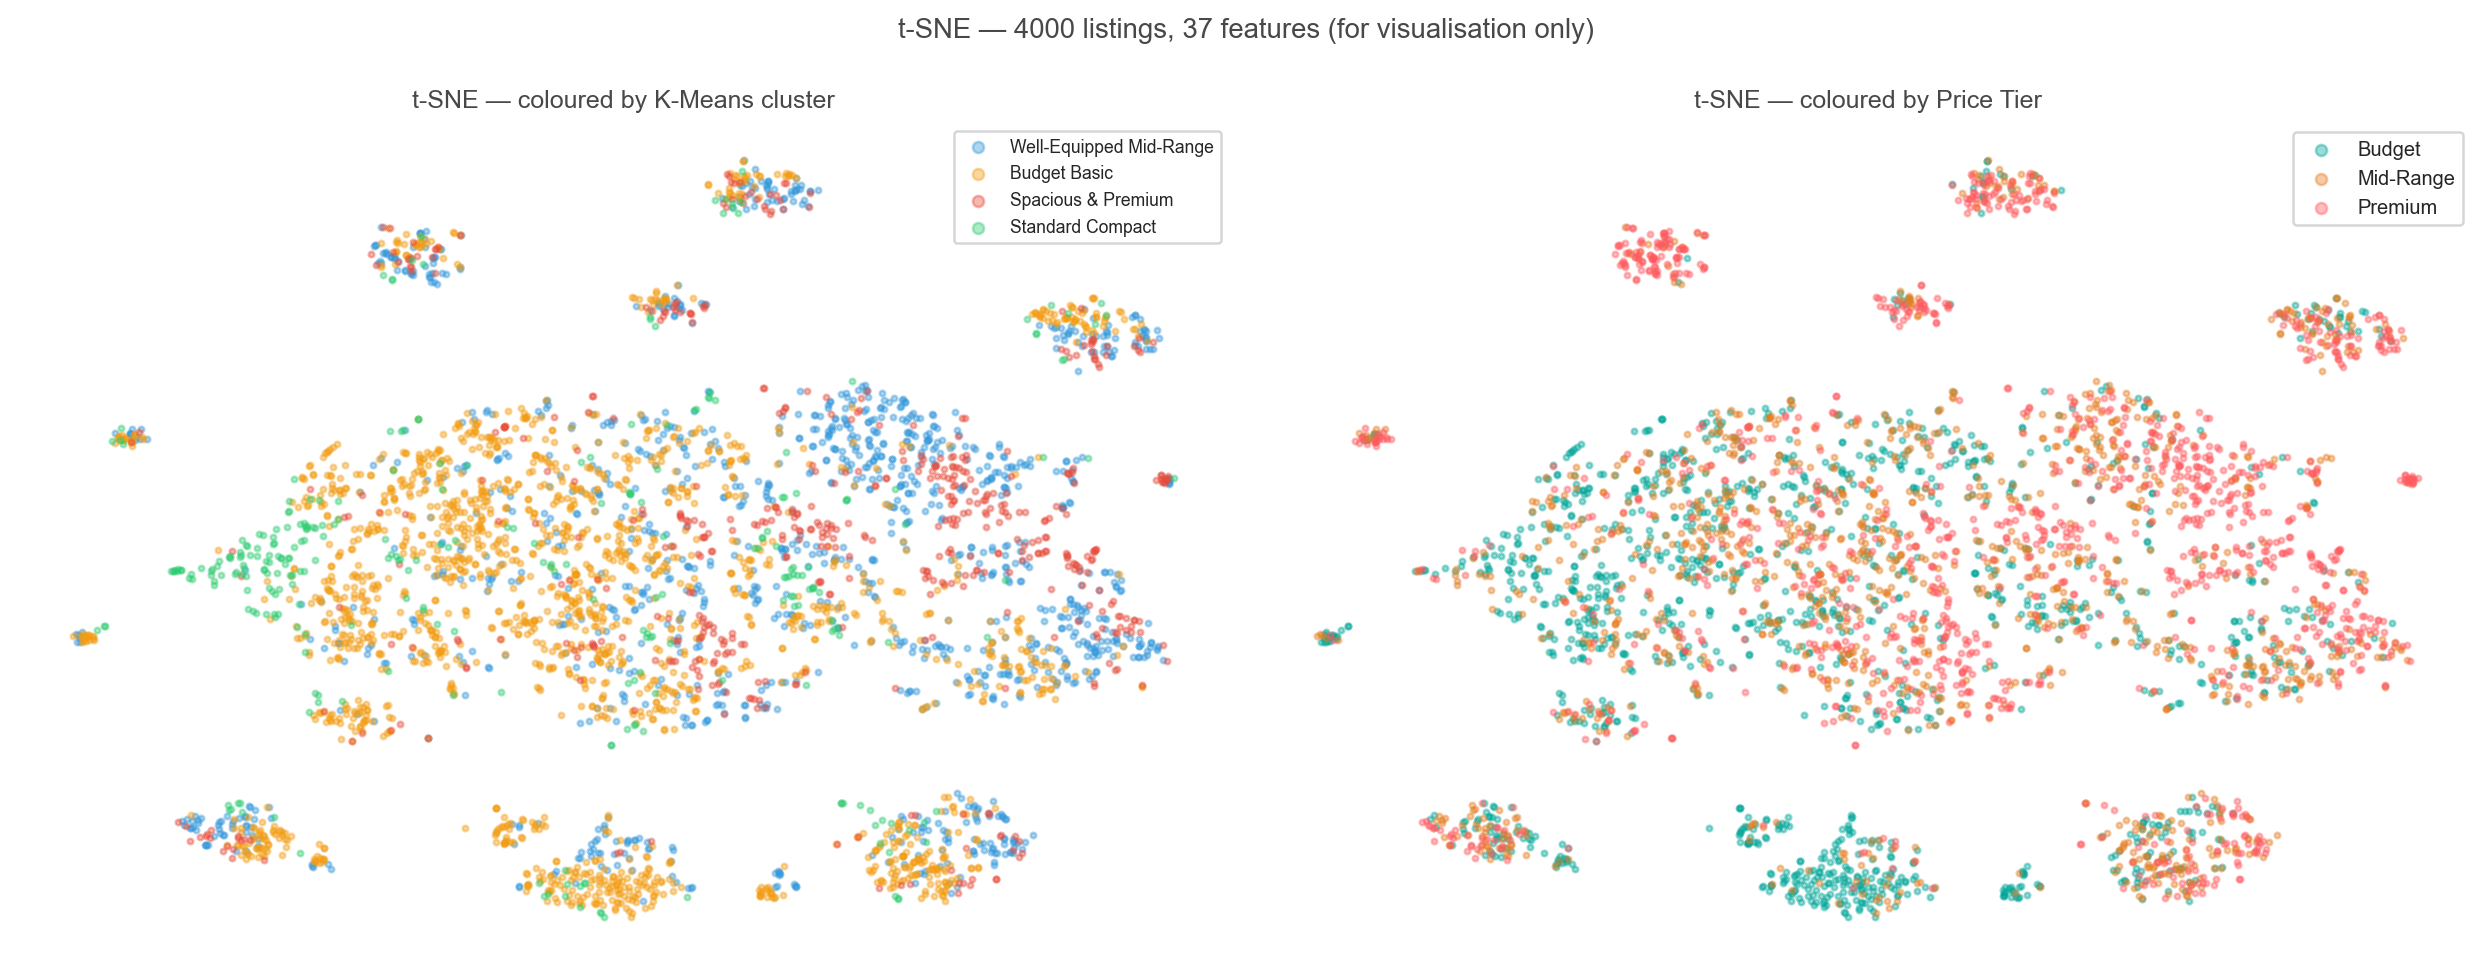
\includegraphics[width=\linewidth]{tsne.png}
  \end{columns}
  \vspace{0.03cm}
  \parbox{\linewidth}{\scriptsize\textcolor{airbnbGrey}{%
    \textbf{Left:} PCA --- 6 clustering features $\rightarrow$ 2 dimensions (linear).
    \textbf{Right:} t-SNE --- full 37-feature space, coloured by cluster (top) and price tier (bottom).
    Both show meaningful separation. Note: t-SNE inter-cluster distances are not interpretable.}}
\end{frame}

\begin{frame}{Geographic Distribution of Clusters}
  \begin{columns}[T]
    \column{0.54\textwidth}
    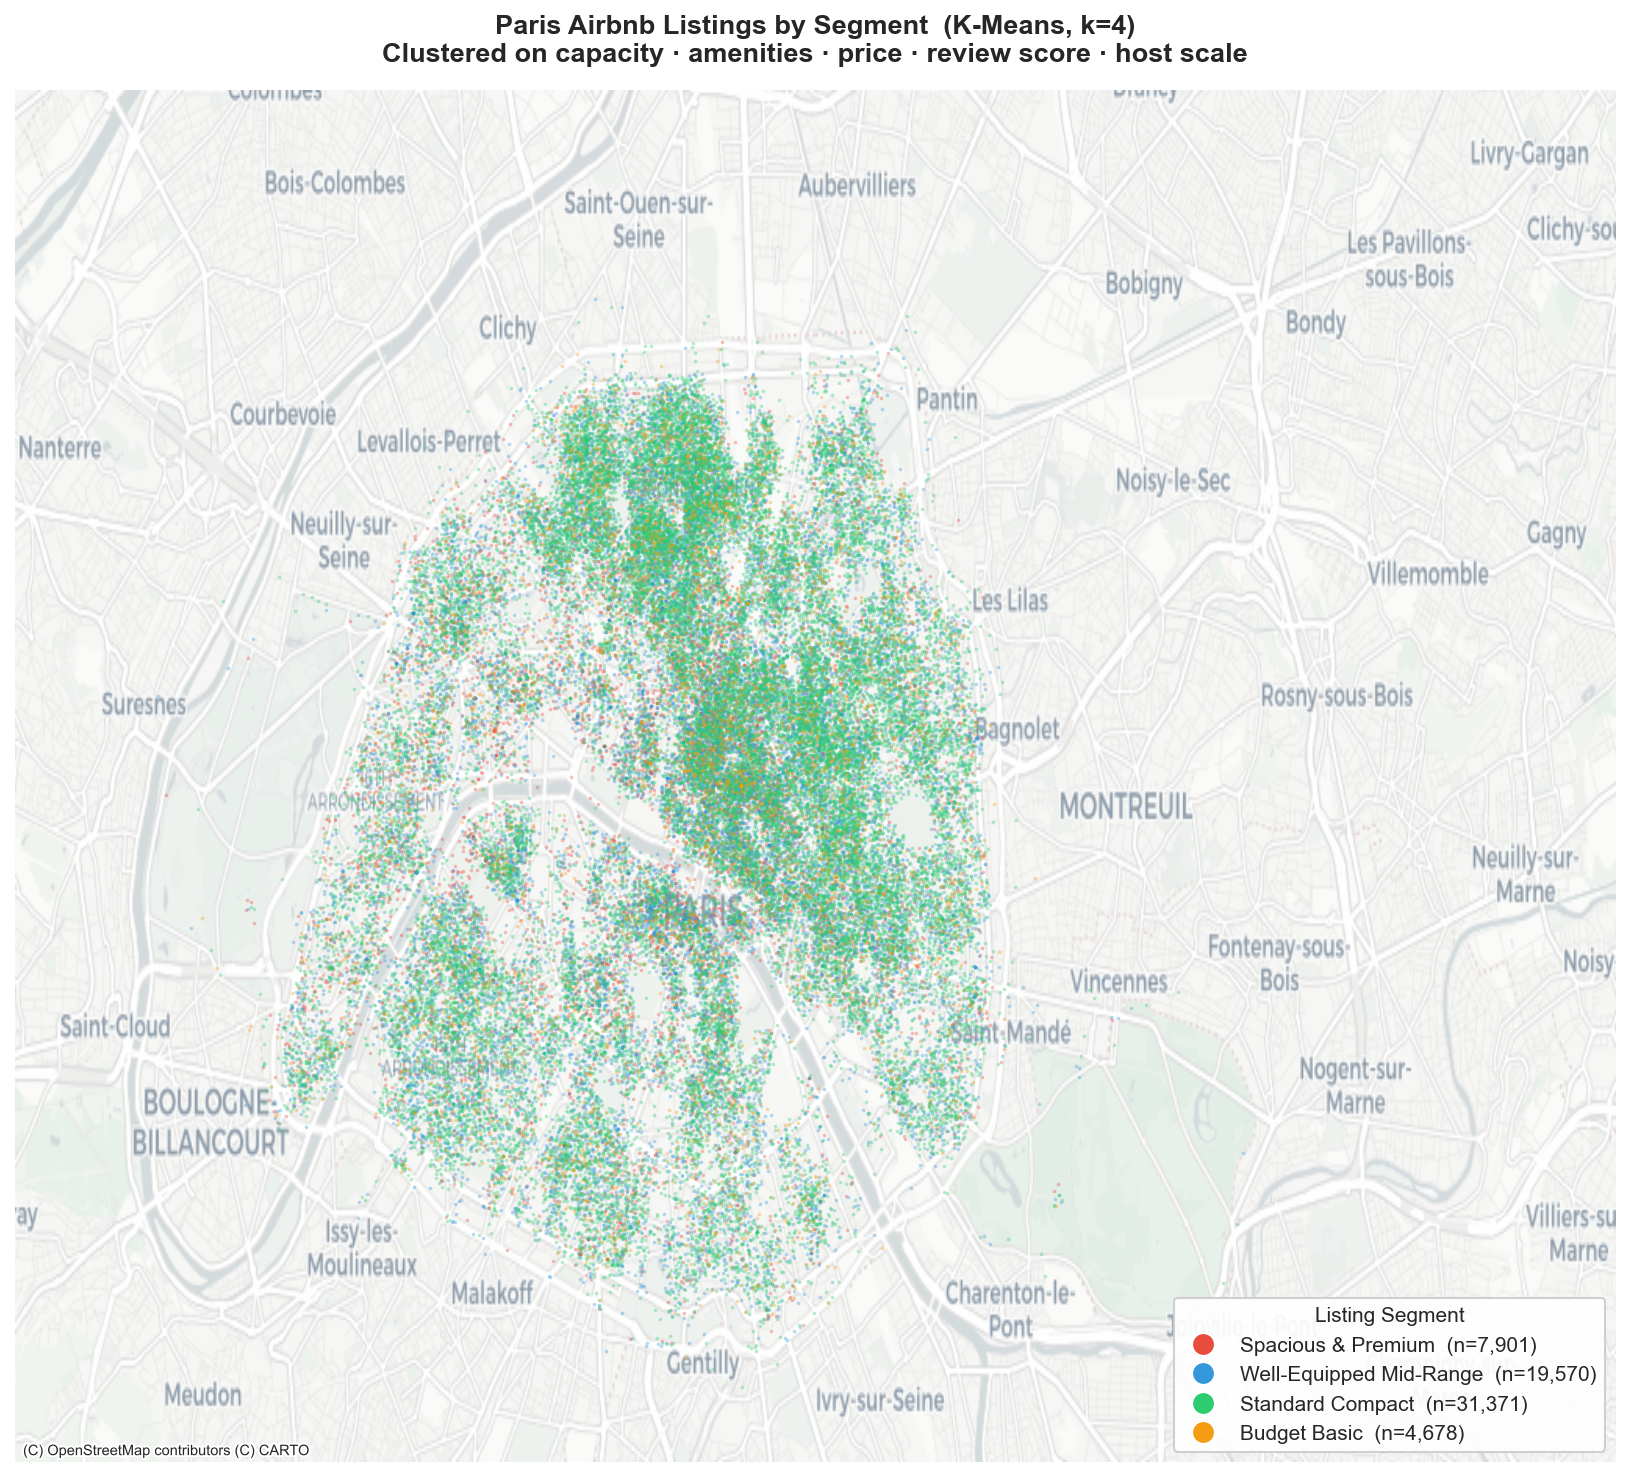
\includegraphics[width=\linewidth, height=0.72\textheight, keepaspectratio]{cluster_map_paris.png}
    \column{0.44\textwidth}
    \small
    \textbf{Spatial patterns}
    \begin{itemize}\setlength{\itemsep}{0.3em}
      \item \textcolor{clusterRed}{\textbf{Spacious \& Premium}} concentrated in\\
            the 7\textsuperscript{e}--8\textsuperscript{e} and 16\textsuperscript{e}
      \item \textcolor{clusterBlue}{\textbf{Mid-Range}} spread across central areas
      \item \textcolor{clusterGreen}{\textbf{Standard Compact}} dominates all\\
            neighbourhoods --- the \hl{typical Paris listing}
      \item \textcolor{clusterOrange}{\textbf{Budget Basic}} scattered,\\
            slightly more on the periphery
    \end{itemize}
    \vspace{0.2cm}
    \parbox{\linewidth}{\scriptsize\textcolor{airbnbGrey}{%
      Clusters were \textbf{not} computed on location features.
      The geographic pattern emerges purely from property characteristics,
      independently confirming the location-price correlation seen in EDA.}}
  \end{columns}
\end{frame}

% ============================================================
\section{Business Recommendations}
% ============================================================

\begin{frame}[shrink=10]{Business Recommendations for Parisian Hosts}
  \begin{columns}[T]
    \column{0.52\textwidth}
    \begin{enumerate}
      \setlength{\itemsep}{0.4em}
      \item[\hl{\faHome}] \textbf{Invest in capacity and amenities}\\
        \small Each extra guest slot and key amenity (elevator, A/C,
        dishwasher) carries a measurable price premium.

      \item[\hl{\faMapMarker}] \textbf{Benchmark against your neighbourhood}\\
        \small Location drives the largest unexplained variance;
        compare to the arrondissement median.

      \item[\hl{\faRobot}] \textbf{Use the predictive model}\\
        \small Tuned XGBoost predicts within \textbf{\texteuro27} on average
        --- query it with your listing's features.

      \item[\hl{\faStar}] \textbf{Maintain review quality}\\
        \small Recent reviews and high ratings sustain price premium.

      \item[\hl{\faLayerGroup}] \textbf{Know your competitive segment}\\
        \small Identify your K-Means cluster to understand your
        direct competitors and price accordingly.
    \end{enumerate}

    \column{0.46\textwidth}
    \begin{block}{Limitations}
      \small\begin{itemize}\setlength{\itemsep}{0.15em}
        \item Static snapshot --- seasonality needs calendar data
        \item Predicts listed price, not realised revenue
        \item Some spec features absent (beds, bathrooms)
        \item No review text --- NLP sentiment infeasible
      \end{itemize}
    \end{block}
    \vspace{0.3cm}
    \begin{block}{Summary}
      \scriptsize
      \begin{tabular}{ll}
        \toprule
        Best model & Tuned XGBoost\\
        Test R\textsuperscript{2} & \textbf{0.658}\\
        RMSE / MAE & \texteuro47.2 / \texteuro27.2\\
        \#1 driver & \texttt{bedrooms} (RF 44\%)\\
        \#2 driver & \texttt{accommodates} ($r$=0.54)\\
        Segments & 4 clusters (K-Means)\\
        Clustering validation & 78\% Ward agreement\\
        \bottomrule
      \end{tabular}
    \end{block}
  \end{columns}
\end{frame}

% ── Closing ─────────────────────────────────────────────────
{
\setbeamercolor{background canvas}{bg=airbnbDark}
\begin{frame}[plain]
  \vspace{1.5cm}
  \begin{center}
    {\color{airbnbCoral}\rule{0.6\textwidth}{2pt}}\\[0.6cm]
    {\color{white}\Large\textbf{Thank you}}\\[0.3cm]
    {\color{airbnbLight}\normalsize Questions welcome}\\[0.8cm]
    {\color{airbnbCoral}\rule{0.6\textwidth}{2pt}}\\[0.5cm]
    {\color{airbnbGrey}\small
      Data: Inside Airbnb (CC0) $\cdot$
      HEC Paris --- Business Analytics Using Python $\cdot$
      Prof.\ Xitong LI}
  \end{center}
\end{frame}
}

\end{document}
